%!TEX root = main.tex
\subsection{Choosing Instrumental Variables Example}
\label{sec:chooseIVsim}
I now evaluate the performance of FMSC in the Instrument Selection Example described in Section \ref{sec:chooseIVexample} using the following simulation design:
\begin{eqnarray}
		y_i &=& 0.5 x_i + \epsilon_i\\ 
		\label{eq:chooseIVDGP1}
		x_i &=& (z_{1i} + z_{2i} + z_{3i}) /3 + \gamma w_i + v_i 
		\label{eq:chooseIVDGP2}
	\end{eqnarray}
for $i=1, 2, \hdots, N$ where $(\epsilon_i, v_i, w_i, z_{i1}, z_{2i}, z_{3i})' \sim \mbox{ iid  } N(0,\mathcal{V})$ with

\begin{equation}	
	\mathcal{V} = \left[  \begin{array}
		{cc} \mathcal{V}_1 & 0 \\ 0 & \mathcal{V}_2
	\end{array}\right], \quad
	\mathcal{V}_1 = \left[ \begin{array}
		{ccc} 
		1 & (0.5 - \gamma \rho) & \rho \\
		(0.5 - \gamma \rho) & (8/9 - \gamma^2) & 0\\ 
		\rho & 0 & 1 \\ 
	\end{array} \right], \quad \mathcal{V}_2 = I_3 / 3
	\label{eq:chooseIVDGP3}
\end{equation}
This setup keeps the variance of $x$ fixed at one and the endogeneity of $x$, $Cor(x, \epsilon)$, fixed at $0.5$ while allowing the relevance, $\gamma = Cor(x,w)$, and endogeneity, $\rho = Cor(w, \epsilon)$, of the instrument $w$ to vary.
The instruments $z_1, z_2, z_3$ are valid and exogenous: they have first-stage coefficients of $1/3$ and are uncorrelated with the second stage error $\epsilon$.
The additional instrument $w$ is only relevant if $\gamma \neq 0$ and is only exogenous if $\rho = 0$.
Since $x$ has unit variance, the first-stage R-squared for this simulation design is simply $1 - \sigma_v^2 = 1/9 + \gamma^2$.
Hence, when  $\gamma = 0$, so that $w$ is irrelevant, the first-stage R-squared is just over 0.11.
Increasing $\gamma$ increases the R-squared of the first-stage.
When $\gamma = 0$, this simulation design is a special case of the DGP used in the Section \ref{sec:OLSvsIVsim}.

As in Section \ref{sec:OLSvsIVsim}, the goal of moment selection in this exercise is to estimate the effect of $x$ on $y$, as before 0.5, with minimum MSE.
In this case, however, the choice is between two TSLS estimators rather than OLS and TSLS: the \emph{valid} estimator uses only $z_1, z_2,$ and $z_3$ as instruments, while the \emph{full} estimator uses $z_1, z_2, z_3,$ and $w$.
The inclusion of $z_1, z_2$ and $z_3$ in both moment sets means that the order of over-identification is two for the valid estimator and three for the full estimator. 
Because the moments of the TSLS estimator only exist up to the order of over-identification \citep{Phillips1980}, this ensures that the small-sample MSE is well-defined.\footnote{Alternatively, one could use fewer instruments for the valid estimator and compare the results using \emph{trimmed} MSE, as in \cite{Hansen2013}.}
All estimators in this section are calculated via TSLS without a constant term using the expressions from Section \ref{sec:chooseIVexample} and 20,000 simulation replications.
 
Figure \ref{fig:chooseIVsim_RMSEbaseline} presents RMSE values for the valid estimator, the full estimator, and the post-FMSC estimator for various combinations of $\gamma$, $\rho$, and $N$.
The results are broadly similar to those from the OLS versus TSLS example presented in Figure \ref{fig:OLSvsIV_RMSEbaseline}.
For any combination $(\gamma,N)$ there is a positive value of $\rho$ below which the full estimator yields a lower RMSE than the full estimator.
As the sample size increases, this cutoff becomes smaller; as $\gamma$ increases, it becomes larger.
As in the OLS versus TSLS example, the post-FMSC estimator represents a compromise between the two estimators over which the FMSC selects.
Unlike in the previous example, however, when $N$ is sufficiently small there is a range of values for $\rho$ within which the FMSC yields a lower RMSE than \emph{both} the valid and full estimators.
This comes from the fact that the valid estimator is quite erratic for small sample sizes: even with 20,000 simulation replications it exhibits a noticable degree of simulation error for $N=50$.
Such behavior is unsurprising given that its first stage is not especially strong, $\mbox{R-squared}\approx 11\%$, and it has only two moments.
In contrast, the full estimator has three moments and a stronger first stage.
As in the OLS versus TSLS example, the post-FMSC estimator does not uniformly outperform the valid estimator for all parameter values, although it does for smaller sample sizes.
The FMSC never performs substantially worse than the valid estimator, however, and often performs dramatically better.
Again, the gains are particularly large for small sample sizes.
\begin{figure}
\centering
	% Created by tikzDevice version 0.7.0 on 2014-07-29 02:49:42
% !TEX encoding = UTF-8 Unicode
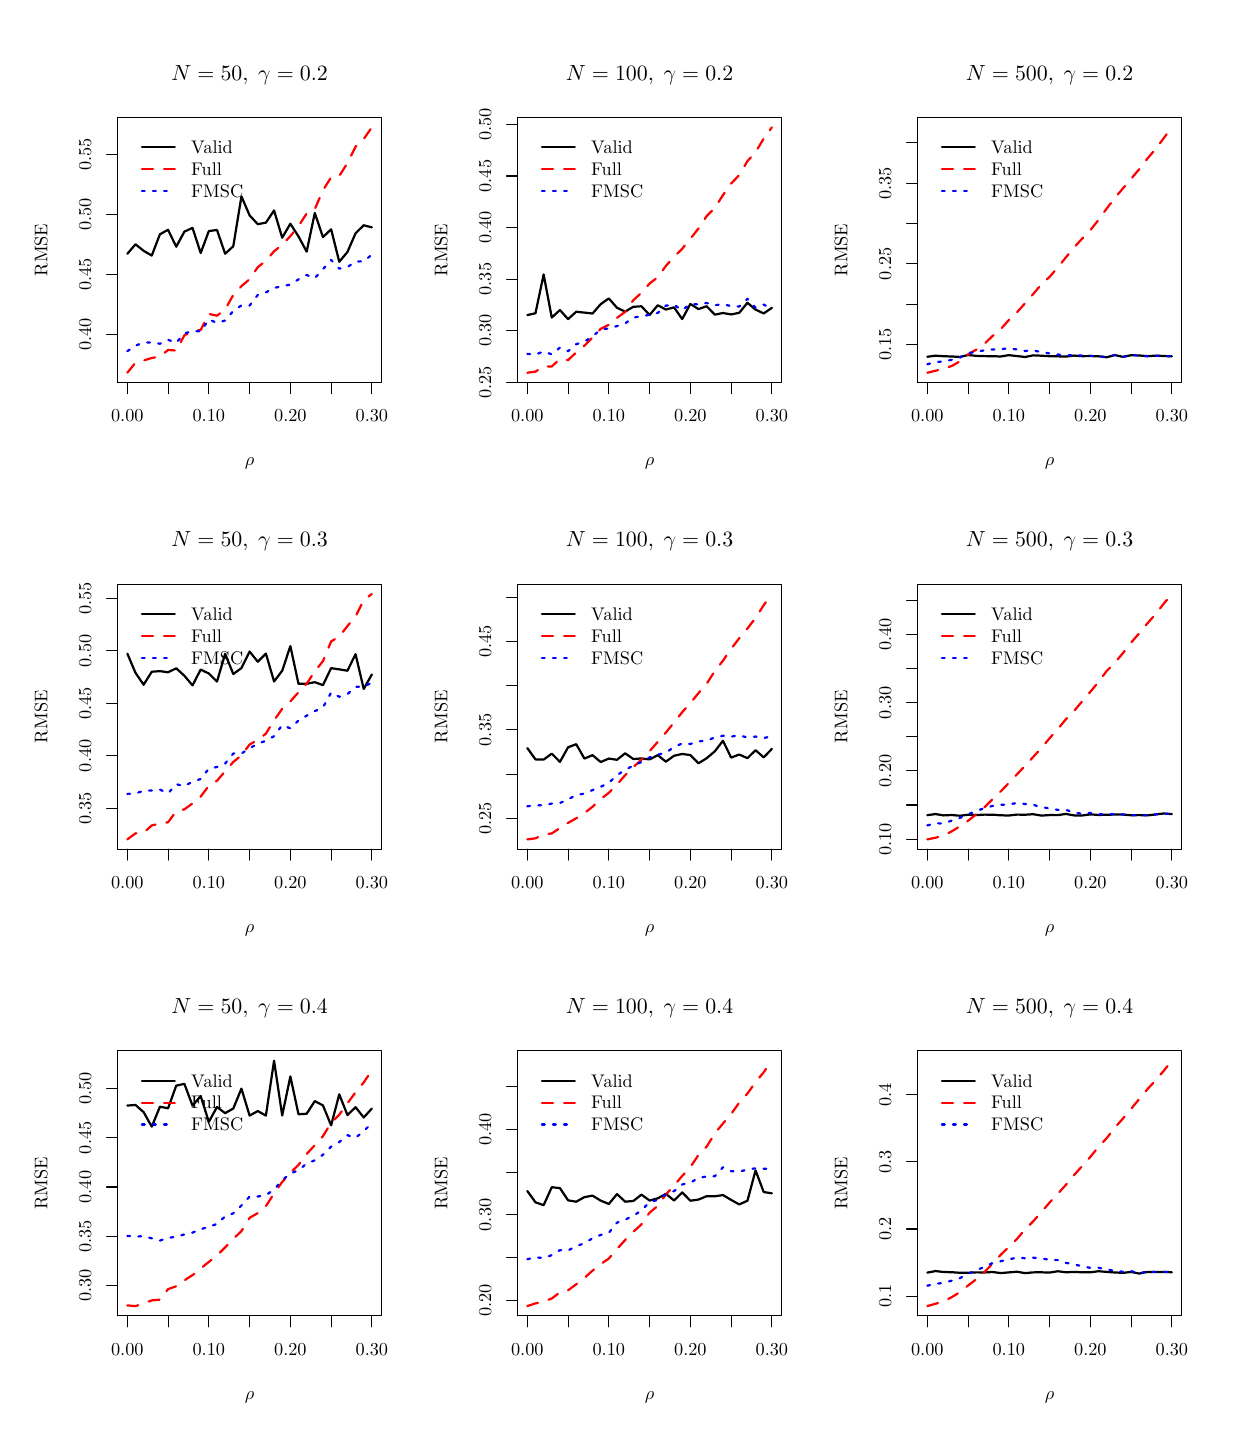
\begin{tikzpicture}[x=1pt,y=1pt]
\definecolor[named]{fillColor}{rgb}{1.00,1.00,1.00}
\path[use as bounding box,fill=fillColor,fill opacity=0.00] (0,0) rectangle (433.62,505.89);
\begin{scope}
\path[clip] ( 32.47,377.65) rectangle (127.91,473.42);
\definecolor[named]{drawColor}{rgb}{0.00,0.00,0.00}

\path[draw=drawColor,line width= 0.8pt,line join=round,line cap=round] ( 36.01,424.15) --
	( 38.95,427.61) --
	( 41.90,425.26) --
	( 44.84,423.54) --
	( 47.79,431.23) --
	( 50.73,432.85) --
	( 53.68,426.73) --
	( 56.63,432.19) --
	( 59.57,433.54) --
	( 62.52,424.45) --
	( 65.46,432.38) --
	( 68.41,432.79) --
	( 71.35,424.19) --
	( 74.30,426.91) --
	( 77.24,444.92) --
	( 80.19,438.07) --
	( 83.14,434.88) --
	( 86.08,435.43) --
	( 89.03,439.83) --
	( 91.97,430.00) --
	( 94.92,435.03) --
	( 97.86,430.45) --
	(100.81,424.95) --
	(103.75,438.92) --
	(106.70,430.21) --
	(109.65,433.03) --
	(112.59,421.28) --
	(115.54,424.82) --
	(118.48,431.58) --
	(121.43,434.49) --
	(124.37,433.72);
\end{scope}
\begin{scope}
\path[clip] (  0.00,  0.00) rectangle (433.62,505.89);
\definecolor[named]{drawColor}{rgb}{0.00,0.00,0.00}

\path[draw=drawColor,line width= 0.4pt,line join=round,line cap=round] ( 36.01,377.65) -- (124.37,377.65);

\path[draw=drawColor,line width= 0.4pt,line join=round,line cap=round] ( 36.01,377.65) -- ( 36.01,373.69);

\path[draw=drawColor,line width= 0.4pt,line join=round,line cap=round] ( 50.73,377.65) -- ( 50.73,373.69);

\path[draw=drawColor,line width= 0.4pt,line join=round,line cap=round] ( 65.46,377.65) -- ( 65.46,373.69);

\path[draw=drawColor,line width= 0.4pt,line join=round,line cap=round] ( 80.19,377.65) -- ( 80.19,373.69);

\path[draw=drawColor,line width= 0.4pt,line join=round,line cap=round] ( 94.92,377.65) -- ( 94.92,373.69);

\path[draw=drawColor,line width= 0.4pt,line join=round,line cap=round] (109.65,377.65) -- (109.65,373.69);

\path[draw=drawColor,line width= 0.4pt,line join=round,line cap=round] (124.37,377.65) -- (124.37,373.69);

\node[text=drawColor,anchor=base,inner sep=0pt, outer sep=0pt, scale=  0.66] at ( 36.01,363.40) {0.00};

\node[text=drawColor,anchor=base,inner sep=0pt, outer sep=0pt, scale=  0.66] at ( 65.46,363.40) {0.10};

\node[text=drawColor,anchor=base,inner sep=0pt, outer sep=0pt, scale=  0.66] at ( 94.92,363.40) {0.20};

\node[text=drawColor,anchor=base,inner sep=0pt, outer sep=0pt, scale=  0.66] at (124.37,363.40) {0.30};

\path[draw=drawColor,line width= 0.4pt,line join=round,line cap=round] ( 32.47,394.97) -- ( 32.47,460.08);

\path[draw=drawColor,line width= 0.4pt,line join=round,line cap=round] ( 32.47,394.97) -- ( 28.51,394.97);

\path[draw=drawColor,line width= 0.4pt,line join=round,line cap=round] ( 32.47,416.68) -- ( 28.51,416.68);

\path[draw=drawColor,line width= 0.4pt,line join=round,line cap=round] ( 32.47,438.38) -- ( 28.51,438.38);

\path[draw=drawColor,line width= 0.4pt,line join=round,line cap=round] ( 32.47,460.08) -- ( 28.51,460.08);

\node[text=drawColor,rotate= 90.00,anchor=base,inner sep=0pt, outer sep=0pt, scale=  0.66] at ( 22.97,394.97) {0.40};

\node[text=drawColor,rotate= 90.00,anchor=base,inner sep=0pt, outer sep=0pt, scale=  0.66] at ( 22.97,416.68) {0.45};

\node[text=drawColor,rotate= 90.00,anchor=base,inner sep=0pt, outer sep=0pt, scale=  0.66] at ( 22.97,438.38) {0.50};

\node[text=drawColor,rotate= 90.00,anchor=base,inner sep=0pt, outer sep=0pt, scale=  0.66] at ( 22.97,460.08) {0.55};

\path[draw=drawColor,line width= 0.4pt,line join=round,line cap=round] ( 32.47,377.65) --
	(127.91,377.65) --
	(127.91,473.42) --
	( 32.47,473.42) --
	( 32.47,377.65);
\end{scope}
\begin{scope}
\path[clip] (  0.00,337.26) rectangle (144.54,505.89);
\definecolor[named]{drawColor}{rgb}{0.00,0.00,0.00}

\node[text=drawColor,anchor=base,inner sep=0pt, outer sep=0pt, scale=  0.79] at ( 80.19,486.92) {\bfseries $N=50, \;\gamma=0.2$};

\node[text=drawColor,anchor=base,inner sep=0pt, outer sep=0pt, scale=  0.66] at ( 80.19,347.56) {$\rho$};

\node[text=drawColor,rotate= 90.00,anchor=base,inner sep=0pt, outer sep=0pt, scale=  0.66] at (  7.13,425.53) {RMSE};
\end{scope}
\begin{scope}
\path[clip] ( 32.47,377.65) rectangle (127.91,473.42);
\definecolor[named]{drawColor}{rgb}{1.00,0.00,0.00}

\path[draw=drawColor,line width= 0.8pt,dash pattern=on 4pt off 4pt ,line join=round,line cap=round] ( 36.01,381.20) --
	( 38.95,384.82) --
	( 41.90,385.63) --
	( 44.84,386.53) --
	( 47.79,387.02) --
	( 50.73,389.43) --
	( 53.68,389.21) --
	( 56.63,394.72) --
	( 59.57,396.22) --
	( 62.52,396.63) --
	( 65.46,402.46) --
	( 68.41,401.81) --
	( 71.35,404.07) --
	( 74.30,409.29) --
	( 77.24,412.47) --
	( 80.19,414.99) --
	( 83.14,419.35) --
	( 86.08,421.65) --
	( 89.03,425.08) --
	( 91.97,427.42) --
	( 94.92,430.56) --
	( 97.86,434.17) --
	(100.81,438.75) --
	(103.75,440.32) --
	(106.70,447.14) --
	(109.65,451.81) --
	(112.59,452.27) --
	(115.54,456.97) --
	(118.48,462.88) --
	(121.43,465.66) --
	(124.37,469.87);
\definecolor[named]{drawColor}{rgb}{0.00,0.00,1.00}

\path[draw=drawColor,line width= 0.8pt,dash pattern=on 1pt off 3pt ,line join=round,line cap=round] ( 36.01,388.99) --
	( 38.95,390.97) --
	( 41.90,392.10) --
	( 44.84,392.17) --
	( 47.79,391.68) --
	( 50.73,393.09) --
	( 53.68,392.01) --
	( 56.63,395.37) --
	( 59.57,396.31) --
	( 62.52,396.11) --
	( 65.46,400.43) --
	( 68.41,399.21) --
	( 71.35,400.06) --
	( 74.30,403.53) --
	( 77.24,405.51) --
	( 80.19,405.47) --
	( 83.14,409.29) --
	( 86.08,410.22) --
	( 89.03,411.89) --
	( 91.97,412.38) --
	( 94.92,413.08) --
	( 97.86,414.92) --
	(100.81,416.51) --
	(103.75,415.38) --
	(106.70,418.59) --
	(109.65,421.96) --
	(112.59,418.82) --
	(115.54,419.37) --
	(118.48,421.38) --
	(121.43,421.48) --
	(124.37,423.84);
\definecolor[named]{drawColor}{rgb}{0.00,0.00,0.00}

\path[draw=drawColor,line width= 0.8pt,line join=round,line cap=round] ( 41.28,462.63) -- ( 53.16,462.63);
\definecolor[named]{drawColor}{rgb}{1.00,0.00,0.00}

\path[draw=drawColor,line width= 0.8pt,dash pattern=on 4pt off 4pt ,line join=round,line cap=round] ( 41.28,454.71) -- ( 53.16,454.71);
\definecolor[named]{drawColor}{rgb}{0.00,0.00,1.00}

\path[draw=drawColor,line width= 0.8pt,dash pattern=on 1pt off 3pt ,line join=round,line cap=round] ( 41.28,446.79) -- ( 53.16,446.79);
\definecolor[named]{drawColor}{rgb}{0.00,0.00,0.00}

\node[text=drawColor,anchor=base west,inner sep=0pt, outer sep=0pt, scale=  0.66] at ( 59.10,460.35) {Valid};

\node[text=drawColor,anchor=base west,inner sep=0pt, outer sep=0pt, scale=  0.66] at ( 59.10,452.43) {Full};

\node[text=drawColor,anchor=base west,inner sep=0pt, outer sep=0pt, scale=  0.66] at ( 59.10,444.51) {FMSC};
\end{scope}
\begin{scope}
\path[clip] (177.01,377.65) rectangle (272.45,473.42);
\definecolor[named]{drawColor}{rgb}{0.00,0.00,0.00}

\path[draw=drawColor,line width= 0.8pt,line join=round,line cap=round] (180.55,402.03) --
	(183.49,402.69) --
	(186.44,416.70) --
	(189.38,401.13) --
	(192.33,403.85) --
	(195.27,400.57) --
	(198.22,403.24) --
	(201.17,402.93) --
	(204.11,402.60) --
	(207.06,405.98) --
	(210.00,408.05) --
	(212.95,404.67) --
	(215.89,403.28) --
	(218.84,405.02) --
	(221.78,405.21) --
	(224.73,402.06) --
	(227.68,405.58) --
	(230.62,404.03) --
	(233.57,404.82) --
	(236.51,400.59) --
	(239.46,406.05) --
	(242.40,404.20) --
	(245.35,405.23) --
	(248.29,402.19) --
	(251.24,402.77) --
	(254.19,402.27) --
	(257.13,402.86) --
	(260.08,406.47) --
	(263.02,404.02) --
	(265.97,402.62) --
	(268.91,404.65);
\end{scope}
\begin{scope}
\path[clip] (  0.00,  0.00) rectangle (433.62,505.89);
\definecolor[named]{drawColor}{rgb}{0.00,0.00,0.00}

\path[draw=drawColor,line width= 0.4pt,line join=round,line cap=round] (180.55,377.65) -- (268.91,377.65);

\path[draw=drawColor,line width= 0.4pt,line join=round,line cap=round] (180.55,377.65) -- (180.55,373.69);

\path[draw=drawColor,line width= 0.4pt,line join=round,line cap=round] (195.27,377.65) -- (195.27,373.69);

\path[draw=drawColor,line width= 0.4pt,line join=round,line cap=round] (210.00,377.65) -- (210.00,373.69);

\path[draw=drawColor,line width= 0.4pt,line join=round,line cap=round] (224.73,377.65) -- (224.73,373.69);

\path[draw=drawColor,line width= 0.4pt,line join=round,line cap=round] (239.46,377.65) -- (239.46,373.69);

\path[draw=drawColor,line width= 0.4pt,line join=round,line cap=round] (254.19,377.65) -- (254.19,373.69);

\path[draw=drawColor,line width= 0.4pt,line join=round,line cap=round] (268.91,377.65) -- (268.91,373.69);

\node[text=drawColor,anchor=base,inner sep=0pt, outer sep=0pt, scale=  0.66] at (180.55,363.40) {0.00};

\node[text=drawColor,anchor=base,inner sep=0pt, outer sep=0pt, scale=  0.66] at (210.00,363.40) {0.10};

\node[text=drawColor,anchor=base,inner sep=0pt, outer sep=0pt, scale=  0.66] at (239.46,363.40) {0.20};

\node[text=drawColor,anchor=base,inner sep=0pt, outer sep=0pt, scale=  0.66] at (268.91,363.40) {0.30};

\path[draw=drawColor,line width= 0.4pt,line join=round,line cap=round] (177.01,377.81) -- (177.01,470.89);

\path[draw=drawColor,line width= 0.4pt,line join=round,line cap=round] (177.01,377.81) -- (173.05,377.81);

\path[draw=drawColor,line width= 0.4pt,line join=round,line cap=round] (177.01,396.42) -- (173.05,396.42);

\path[draw=drawColor,line width= 0.4pt,line join=round,line cap=round] (177.01,415.04) -- (173.05,415.04);

\path[draw=drawColor,line width= 0.4pt,line join=round,line cap=round] (177.01,433.66) -- (173.05,433.66);

\path[draw=drawColor,line width= 0.4pt,line join=round,line cap=round] (177.01,452.27) -- (173.05,452.27);

\path[draw=drawColor,line width= 0.4pt,line join=round,line cap=round] (177.01,470.89) -- (173.05,470.89);

\node[text=drawColor,rotate= 90.00,anchor=base,inner sep=0pt, outer sep=0pt, scale=  0.66] at (167.51,377.81) {0.25};

\node[text=drawColor,rotate= 90.00,anchor=base,inner sep=0pt, outer sep=0pt, scale=  0.66] at (167.51,396.42) {0.30};

\node[text=drawColor,rotate= 90.00,anchor=base,inner sep=0pt, outer sep=0pt, scale=  0.66] at (167.51,415.04) {0.35};

\node[text=drawColor,rotate= 90.00,anchor=base,inner sep=0pt, outer sep=0pt, scale=  0.66] at (167.51,433.66) {0.40};

\node[text=drawColor,rotate= 90.00,anchor=base,inner sep=0pt, outer sep=0pt, scale=  0.66] at (167.51,452.27) {0.45};

\node[text=drawColor,rotate= 90.00,anchor=base,inner sep=0pt, outer sep=0pt, scale=  0.66] at (167.51,470.89) {0.50};

\path[draw=drawColor,line width= 0.4pt,line join=round,line cap=round] (177.01,377.65) --
	(272.45,377.65) --
	(272.45,473.42) --
	(177.01,473.42) --
	(177.01,377.65);
\end{scope}
\begin{scope}
\path[clip] (144.54,337.26) rectangle (289.08,505.89);
\definecolor[named]{drawColor}{rgb}{0.00,0.00,0.00}

\node[text=drawColor,anchor=base,inner sep=0pt, outer sep=0pt, scale=  0.79] at (224.73,486.92) {\bfseries $N=100, \;\gamma=0.2$};

\node[text=drawColor,anchor=base,inner sep=0pt, outer sep=0pt, scale=  0.66] at (224.73,347.56) {$\rho$};

\node[text=drawColor,rotate= 90.00,anchor=base,inner sep=0pt, outer sep=0pt, scale=  0.66] at (151.67,425.53) {RMSE};
\end{scope}
\begin{scope}
\path[clip] (177.01,377.65) rectangle (272.45,473.42);
\definecolor[named]{drawColor}{rgb}{1.00,0.00,0.00}

\path[draw=drawColor,line width= 0.8pt,dash pattern=on 4pt off 4pt ,line join=round,line cap=round] (180.55,381.20) --
	(183.49,381.58) --
	(186.44,383.54) --
	(189.38,383.44) --
	(192.33,386.21) --
	(195.27,385.76) --
	(198.22,388.57) --
	(201.17,390.96) --
	(204.11,393.95) --
	(207.06,397.06) --
	(210.00,398.51) --
	(212.95,401.03) --
	(215.89,403.20) --
	(218.84,407.40) --
	(221.78,410.07) --
	(224.73,413.43) --
	(227.68,415.73) --
	(230.62,419.81) --
	(233.57,423.09) --
	(236.51,425.98) --
	(239.46,429.63) --
	(242.40,433.31) --
	(245.35,437.80) --
	(248.29,440.75) --
	(251.24,445.38) --
	(254.19,449.54) --
	(257.13,452.66) --
	(260.08,457.65) --
	(263.02,460.92) --
	(265.97,465.81) --
	(268.91,469.87);
\definecolor[named]{drawColor}{rgb}{0.00,0.00,1.00}

\path[draw=drawColor,line width= 0.8pt,dash pattern=on 1pt off 3pt ,line join=round,line cap=round] (180.55,388.00) --
	(183.49,387.77) --
	(186.44,388.89) --
	(189.38,387.83) --
	(192.33,390.28) --
	(195.27,388.99) --
	(198.22,391.51) --
	(201.17,392.44) --
	(204.11,394.33) --
	(207.06,396.81) --
	(210.00,397.22) --
	(212.95,398.05) --
	(215.89,399.02) --
	(218.84,401.12) --
	(221.78,401.60) --
	(224.73,402.12) --
	(227.68,402.81) --
	(230.62,405.46) --
	(233.57,405.72) --
	(236.51,403.76) --
	(239.46,406.11) --
	(242.40,405.85) --
	(245.35,406.41) --
	(248.29,405.56) --
	(251.24,406.04) --
	(254.19,405.23) --
	(257.13,405.15) --
	(260.08,407.91) --
	(263.02,404.68) --
	(265.97,405.82) --
	(268.91,404.25);
\definecolor[named]{drawColor}{rgb}{0.00,0.00,0.00}

\path[draw=drawColor,line width= 0.8pt,line join=round,line cap=round] (185.82,462.63) -- (197.70,462.63);
\definecolor[named]{drawColor}{rgb}{1.00,0.00,0.00}

\path[draw=drawColor,line width= 0.8pt,dash pattern=on 4pt off 4pt ,line join=round,line cap=round] (185.82,454.71) -- (197.70,454.71);
\definecolor[named]{drawColor}{rgb}{0.00,0.00,1.00}

\path[draw=drawColor,line width= 0.8pt,dash pattern=on 1pt off 3pt ,line join=round,line cap=round] (185.82,446.79) -- (197.70,446.79);
\definecolor[named]{drawColor}{rgb}{0.00,0.00,0.00}

\node[text=drawColor,anchor=base west,inner sep=0pt, outer sep=0pt, scale=  0.66] at (203.64,460.35) {Valid};

\node[text=drawColor,anchor=base west,inner sep=0pt, outer sep=0pt, scale=  0.66] at (203.64,452.43) {Full};

\node[text=drawColor,anchor=base west,inner sep=0pt, outer sep=0pt, scale=  0.66] at (203.64,444.51) {FMSC};
\end{scope}
\begin{scope}
\path[clip] (321.55,377.65) rectangle (416.99,473.42);
\definecolor[named]{drawColor}{rgb}{0.00,0.00,0.00}

\path[draw=drawColor,line width= 0.8pt,line join=round,line cap=round] (325.09,386.97) --
	(328.03,387.36) --
	(330.98,387.16) --
	(333.92,387.07) --
	(336.87,386.91) --
	(339.81,387.59) --
	(342.76,387.30) --
	(345.71,387.20) --
	(348.65,387.17) --
	(351.60,387.07) --
	(354.54,387.55) --
	(357.49,387.22) --
	(360.43,386.89) --
	(363.38,387.48) --
	(366.32,387.35) --
	(369.27,387.16) --
	(372.22,387.12) --
	(375.16,387.03) --
	(378.11,387.39) --
	(381.05,387.18) --
	(384.00,387.22) --
	(386.94,387.14) --
	(389.89,386.78) --
	(392.83,387.58) --
	(395.78,386.93) --
	(398.73,387.53) --
	(401.67,387.43) --
	(404.62,387.18) --
	(407.56,387.37) --
	(410.51,387.24) --
	(413.45,387.13);
\end{scope}
\begin{scope}
\path[clip] (  0.00,  0.00) rectangle (433.62,505.89);
\definecolor[named]{drawColor}{rgb}{0.00,0.00,0.00}

\path[draw=drawColor,line width= 0.4pt,line join=round,line cap=round] (325.09,377.65) -- (413.45,377.65);

\path[draw=drawColor,line width= 0.4pt,line join=round,line cap=round] (325.09,377.65) -- (325.09,373.69);

\path[draw=drawColor,line width= 0.4pt,line join=round,line cap=round] (339.81,377.65) -- (339.81,373.69);

\path[draw=drawColor,line width= 0.4pt,line join=round,line cap=round] (354.54,377.65) -- (354.54,373.69);

\path[draw=drawColor,line width= 0.4pt,line join=round,line cap=round] (369.27,377.65) -- (369.27,373.69);

\path[draw=drawColor,line width= 0.4pt,line join=round,line cap=round] (384.00,377.65) -- (384.00,373.69);

\path[draw=drawColor,line width= 0.4pt,line join=round,line cap=round] (398.73,377.65) -- (398.73,373.69);

\path[draw=drawColor,line width= 0.4pt,line join=round,line cap=round] (413.45,377.65) -- (413.45,373.69);

\node[text=drawColor,anchor=base,inner sep=0pt, outer sep=0pt, scale=  0.66] at (325.09,363.40) {0.00};

\node[text=drawColor,anchor=base,inner sep=0pt, outer sep=0pt, scale=  0.66] at (354.54,363.40) {0.10};

\node[text=drawColor,anchor=base,inner sep=0pt, outer sep=0pt, scale=  0.66] at (384.00,363.40) {0.20};

\node[text=drawColor,anchor=base,inner sep=0pt, outer sep=0pt, scale=  0.66] at (413.45,363.40) {0.30};

\path[draw=drawColor,line width= 0.4pt,line join=round,line cap=round] (321.55,391.42) -- (321.55,464.29);

\path[draw=drawColor,line width= 0.4pt,line join=round,line cap=round] (321.55,391.42) -- (317.59,391.42);

\path[draw=drawColor,line width= 0.4pt,line join=round,line cap=round] (321.55,405.99) -- (317.59,405.99);

\path[draw=drawColor,line width= 0.4pt,line join=round,line cap=round] (321.55,420.57) -- (317.59,420.57);

\path[draw=drawColor,line width= 0.4pt,line join=round,line cap=round] (321.55,435.14) -- (317.59,435.14);

\path[draw=drawColor,line width= 0.4pt,line join=round,line cap=round] (321.55,449.71) -- (317.59,449.71);

\path[draw=drawColor,line width= 0.4pt,line join=round,line cap=round] (321.55,464.29) -- (317.59,464.29);

\node[text=drawColor,rotate= 90.00,anchor=base,inner sep=0pt, outer sep=0pt, scale=  0.66] at (312.05,391.42) {0.15};

\node[text=drawColor,rotate= 90.00,anchor=base,inner sep=0pt, outer sep=0pt, scale=  0.66] at (312.05,420.57) {0.25};

\node[text=drawColor,rotate= 90.00,anchor=base,inner sep=0pt, outer sep=0pt, scale=  0.66] at (312.05,449.71) {0.35};

\path[draw=drawColor,line width= 0.4pt,line join=round,line cap=round] (321.55,377.65) --
	(416.99,377.65) --
	(416.99,473.42) --
	(321.55,473.42) --
	(321.55,377.65);
\end{scope}
\begin{scope}
\path[clip] (289.08,337.26) rectangle (433.62,505.89);
\definecolor[named]{drawColor}{rgb}{0.00,0.00,0.00}

\node[text=drawColor,anchor=base,inner sep=0pt, outer sep=0pt, scale=  0.79] at (369.27,486.92) {\bfseries $N=500, \;\gamma=0.2$};

\node[text=drawColor,anchor=base,inner sep=0pt, outer sep=0pt, scale=  0.66] at (369.27,347.56) {$\rho$};

\node[text=drawColor,rotate= 90.00,anchor=base,inner sep=0pt, outer sep=0pt, scale=  0.66] at (296.21,425.53) {RMSE};
\end{scope}
\begin{scope}
\path[clip] (321.55,377.65) rectangle (416.99,473.42);
\definecolor[named]{drawColor}{rgb}{1.00,0.00,0.00}

\path[draw=drawColor,line width= 0.8pt,dash pattern=on 4pt off 4pt ,line join=round,line cap=round] (325.09,381.20) --
	(328.03,381.90) --
	(330.98,382.64) --
	(333.92,383.64) --
	(336.87,385.33) --
	(339.81,387.85) --
	(342.76,389.53) --
	(345.71,391.62) --
	(348.65,394.48) --
	(351.60,396.91) --
	(354.54,400.25) --
	(357.49,403.07) --
	(360.43,406.33) --
	(363.38,409.68) --
	(366.32,413.18) --
	(369.27,415.82) --
	(372.22,419.24) --
	(375.16,422.89) --
	(378.11,426.44) --
	(381.05,429.68) --
	(384.00,432.72) --
	(386.94,436.41) --
	(389.89,440.52) --
	(392.83,444.32) --
	(395.78,447.82) --
	(398.73,451.30) --
	(401.67,454.76) --
	(404.62,458.59) --
	(407.56,462.04) --
	(410.51,465.97) --
	(413.45,469.87);
\definecolor[named]{drawColor}{rgb}{0.00,0.00,1.00}

\path[draw=drawColor,line width= 0.8pt,dash pattern=on 1pt off 3pt ,line join=round,line cap=round] (325.09,384.27) --
	(328.03,385.01) --
	(330.98,385.31) --
	(333.92,385.85) --
	(336.87,386.72) --
	(339.81,388.28) --
	(342.76,388.72) --
	(345.71,389.31) --
	(348.65,389.60) --
	(351.60,389.66) --
	(354.54,390.10) --
	(357.49,389.58) --
	(360.43,389.08) --
	(363.38,389.20) --
	(366.32,388.69) --
	(369.27,388.16) --
	(372.22,387.78) --
	(375.16,387.40) --
	(378.11,387.66) --
	(381.05,387.39) --
	(384.00,387.30) --
	(386.94,387.20) --
	(389.89,386.79) --
	(392.83,387.59) --
	(395.78,386.93) --
	(398.73,387.53) --
	(401.67,387.43) --
	(404.62,387.18) --
	(407.56,387.37) --
	(410.51,387.24) --
	(413.45,387.13);
\definecolor[named]{drawColor}{rgb}{0.00,0.00,0.00}

\path[draw=drawColor,line width= 0.8pt,line join=round,line cap=round] (330.36,462.63) -- (342.24,462.63);
\definecolor[named]{drawColor}{rgb}{1.00,0.00,0.00}

\path[draw=drawColor,line width= 0.8pt,dash pattern=on 4pt off 4pt ,line join=round,line cap=round] (330.36,454.71) -- (342.24,454.71);
\definecolor[named]{drawColor}{rgb}{0.00,0.00,1.00}

\path[draw=drawColor,line width= 0.8pt,dash pattern=on 1pt off 3pt ,line join=round,line cap=round] (330.36,446.79) -- (342.24,446.79);
\definecolor[named]{drawColor}{rgb}{0.00,0.00,0.00}

\node[text=drawColor,anchor=base west,inner sep=0pt, outer sep=0pt, scale=  0.66] at (348.18,460.35) {Valid};

\node[text=drawColor,anchor=base west,inner sep=0pt, outer sep=0pt, scale=  0.66] at (348.18,452.43) {Full};

\node[text=drawColor,anchor=base west,inner sep=0pt, outer sep=0pt, scale=  0.66] at (348.18,444.51) {FMSC};
\end{scope}
\begin{scope}
\path[clip] ( 32.47,209.02) rectangle (127.91,304.79);
\definecolor[named]{drawColor}{rgb}{0.00,0.00,0.00}

\path[draw=drawColor,line width= 0.8pt,line join=round,line cap=round] ( 36.01,279.71) --
	( 38.95,272.76) --
	( 41.90,268.46) --
	( 44.84,273.16) --
	( 47.79,273.37) --
	( 50.73,272.95) --
	( 53.68,274.40) --
	( 56.63,271.70) --
	( 59.57,268.22) --
	( 62.52,273.95) --
	( 65.46,272.51) --
	( 68.41,269.58) --
	( 71.35,279.63) --
	( 74.30,272.32) --
	( 77.24,274.48) --
	( 80.19,280.45) --
	( 83.14,276.77) --
	( 86.08,279.72) --
	( 89.03,269.63) --
	( 91.97,273.52) --
	( 94.92,282.41) --
	( 97.86,268.78) --
	(100.81,268.81) --
	(103.75,269.38) --
	(106.70,268.32) --
	(109.65,274.45) --
	(112.59,274.01) --
	(115.54,273.52) --
	(118.48,279.49) --
	(121.43,266.94) --
	(124.37,272.17);
\end{scope}
\begin{scope}
\path[clip] (  0.00,  0.00) rectangle (433.62,505.89);
\definecolor[named]{drawColor}{rgb}{0.00,0.00,0.00}

\path[draw=drawColor,line width= 0.4pt,line join=round,line cap=round] ( 36.01,209.02) -- (124.37,209.02);

\path[draw=drawColor,line width= 0.4pt,line join=round,line cap=round] ( 36.01,209.02) -- ( 36.01,205.06);

\path[draw=drawColor,line width= 0.4pt,line join=round,line cap=round] ( 50.73,209.02) -- ( 50.73,205.06);

\path[draw=drawColor,line width= 0.4pt,line join=round,line cap=round] ( 65.46,209.02) -- ( 65.46,205.06);

\path[draw=drawColor,line width= 0.4pt,line join=round,line cap=round] ( 80.19,209.02) -- ( 80.19,205.06);

\path[draw=drawColor,line width= 0.4pt,line join=round,line cap=round] ( 94.92,209.02) -- ( 94.92,205.06);

\path[draw=drawColor,line width= 0.4pt,line join=round,line cap=round] (109.65,209.02) -- (109.65,205.06);

\path[draw=drawColor,line width= 0.4pt,line join=round,line cap=round] (124.37,209.02) -- (124.37,205.06);

\node[text=drawColor,anchor=base,inner sep=0pt, outer sep=0pt, scale=  0.66] at ( 36.01,194.77) {0.00};

\node[text=drawColor,anchor=base,inner sep=0pt, outer sep=0pt, scale=  0.66] at ( 65.46,194.77) {0.10};

\node[text=drawColor,anchor=base,inner sep=0pt, outer sep=0pt, scale=  0.66] at ( 94.92,194.77) {0.20};

\node[text=drawColor,anchor=base,inner sep=0pt, outer sep=0pt, scale=  0.66] at (124.37,194.77) {0.30};

\path[draw=drawColor,line width= 0.4pt,line join=round,line cap=round] ( 32.47,223.84) -- ( 32.47,299.62);

\path[draw=drawColor,line width= 0.4pt,line join=round,line cap=round] ( 32.47,223.84) -- ( 28.51,223.84);

\path[draw=drawColor,line width= 0.4pt,line join=round,line cap=round] ( 32.47,242.79) -- ( 28.51,242.79);

\path[draw=drawColor,line width= 0.4pt,line join=round,line cap=round] ( 32.47,261.73) -- ( 28.51,261.73);

\path[draw=drawColor,line width= 0.4pt,line join=round,line cap=round] ( 32.47,280.67) -- ( 28.51,280.67);

\path[draw=drawColor,line width= 0.4pt,line join=round,line cap=round] ( 32.47,299.62) -- ( 28.51,299.62);

\node[text=drawColor,rotate= 90.00,anchor=base,inner sep=0pt, outer sep=0pt, scale=  0.66] at ( 22.97,223.84) {0.35};

\node[text=drawColor,rotate= 90.00,anchor=base,inner sep=0pt, outer sep=0pt, scale=  0.66] at ( 22.97,242.79) {0.40};

\node[text=drawColor,rotate= 90.00,anchor=base,inner sep=0pt, outer sep=0pt, scale=  0.66] at ( 22.97,261.73) {0.45};

\node[text=drawColor,rotate= 90.00,anchor=base,inner sep=0pt, outer sep=0pt, scale=  0.66] at ( 22.97,280.67) {0.50};

\node[text=drawColor,rotate= 90.00,anchor=base,inner sep=0pt, outer sep=0pt, scale=  0.66] at ( 22.97,299.62) {0.55};

\path[draw=drawColor,line width= 0.4pt,line join=round,line cap=round] ( 32.47,209.02) --
	(127.91,209.02) --
	(127.91,304.79) --
	( 32.47,304.79) --
	( 32.47,209.02);
\end{scope}
\begin{scope}
\path[clip] (  0.00,168.63) rectangle (144.54,337.26);
\definecolor[named]{drawColor}{rgb}{0.00,0.00,0.00}

\node[text=drawColor,anchor=base,inner sep=0pt, outer sep=0pt, scale=  0.79] at ( 80.19,318.29) {\bfseries $N=50, \;\gamma=0.3$};

\node[text=drawColor,anchor=base,inner sep=0pt, outer sep=0pt, scale=  0.66] at ( 80.19,178.93) {$\rho$};

\node[text=drawColor,rotate= 90.00,anchor=base,inner sep=0pt, outer sep=0pt, scale=  0.66] at (  7.13,256.90) {RMSE};
\end{scope}
\begin{scope}
\path[clip] ( 32.47,209.02) rectangle (127.91,304.79);
\definecolor[named]{drawColor}{rgb}{1.00,0.00,0.00}

\path[draw=drawColor,line width= 0.8pt,dash pattern=on 4pt off 4pt ,line join=round,line cap=round] ( 36.01,212.57) --
	( 38.95,214.75) --
	( 41.90,214.90) --
	( 44.84,217.63) --
	( 47.79,218.28) --
	( 50.73,218.75) --
	( 53.68,222.75) --
	( 56.63,223.43) --
	( 59.57,225.59) --
	( 62.52,228.05) --
	( 65.46,231.95) --
	( 68.41,233.76) --
	( 71.35,237.19) --
	( 74.30,240.56) --
	( 77.24,242.94) --
	( 80.19,246.86) --
	( 83.14,248.52) --
	( 86.08,250.79) --
	( 89.03,255.59) --
	( 91.97,259.76) --
	( 94.92,262.43) --
	( 97.86,265.74) --
	(100.81,268.82) --
	(103.75,273.30) --
	(106.70,276.98) --
	(109.65,284.09) --
	(112.59,285.89) --
	(115.54,289.65) --
	(118.48,293.08) --
	(121.43,299.01) --
	(124.37,301.24);
\definecolor[named]{drawColor}{rgb}{0.00,0.00,1.00}

\path[draw=drawColor,line width= 0.8pt,dash pattern=on 1pt off 3pt ,line join=round,line cap=round] ( 36.01,228.99) --
	( 38.95,229.22) --
	( 41.90,230.08) --
	( 44.84,230.24) --
	( 47.79,230.56) --
	( 50.73,229.22) --
	( 53.68,232.50) --
	( 56.63,231.84) --
	( 59.57,233.42) --
	( 62.52,234.39) --
	( 65.46,238.13) --
	( 68.41,238.74) --
	( 71.35,239.99) --
	( 74.30,243.59) --
	( 77.24,243.60) --
	( 80.19,245.51) --
	( 83.14,247.14) --
	( 86.08,248.20) --
	( 89.03,249.87) --
	( 91.97,253.86) --
	( 94.92,252.70) --
	( 97.86,255.53) --
	(100.81,257.28) --
	(103.75,258.92) --
	(106.70,260.25) --
	(109.65,265.62) --
	(112.59,264.11) --
	(115.54,265.05) --
	(118.48,267.68) --
	(121.43,267.82) --
	(124.37,269.14);
\definecolor[named]{drawColor}{rgb}{0.00,0.00,0.00}

\path[draw=drawColor,line width= 0.8pt,line join=round,line cap=round] ( 41.28,294.00) -- ( 53.16,294.00);
\definecolor[named]{drawColor}{rgb}{1.00,0.00,0.00}

\path[draw=drawColor,line width= 0.8pt,dash pattern=on 4pt off 4pt ,line join=round,line cap=round] ( 41.28,286.08) -- ( 53.16,286.08);
\definecolor[named]{drawColor}{rgb}{0.00,0.00,1.00}

\path[draw=drawColor,line width= 0.8pt,dash pattern=on 1pt off 3pt ,line join=round,line cap=round] ( 41.28,278.16) -- ( 53.16,278.16);
\definecolor[named]{drawColor}{rgb}{0.00,0.00,0.00}

\node[text=drawColor,anchor=base west,inner sep=0pt, outer sep=0pt, scale=  0.66] at ( 59.10,291.72) {Valid};

\node[text=drawColor,anchor=base west,inner sep=0pt, outer sep=0pt, scale=  0.66] at ( 59.10,283.80) {Full};

\node[text=drawColor,anchor=base west,inner sep=0pt, outer sep=0pt, scale=  0.66] at ( 59.10,275.88) {FMSC};
\end{scope}
\begin{scope}
\path[clip] (177.01,209.02) rectangle (272.45,304.79);
\definecolor[named]{drawColor}{rgb}{0.00,0.00,0.00}

\path[draw=drawColor,line width= 0.8pt,line join=round,line cap=round] (180.55,245.57) --
	(183.49,241.48) --
	(186.44,241.41) --
	(189.38,243.55) --
	(192.33,240.58) --
	(195.27,245.86) --
	(198.22,246.97) --
	(201.17,241.78) --
	(204.11,243.01) --
	(207.06,240.53) --
	(210.00,241.78) --
	(212.95,241.33) --
	(215.89,243.69) --
	(218.84,241.62) --
	(221.78,241.81) --
	(224.73,241.48) --
	(227.68,243.01) --
	(230.62,240.66) --
	(233.57,242.80) --
	(236.51,243.44) --
	(239.46,243.04) --
	(242.40,240.08) --
	(245.35,241.90) --
	(248.29,244.40) --
	(251.24,248.20) --
	(254.19,242.13) --
	(257.13,243.23) --
	(260.08,241.93) --
	(263.02,244.80) --
	(265.97,242.20) --
	(268.91,245.28);
\end{scope}
\begin{scope}
\path[clip] (  0.00,  0.00) rectangle (433.62,505.89);
\definecolor[named]{drawColor}{rgb}{0.00,0.00,0.00}

\path[draw=drawColor,line width= 0.4pt,line join=round,line cap=round] (180.55,209.02) -- (268.91,209.02);

\path[draw=drawColor,line width= 0.4pt,line join=round,line cap=round] (180.55,209.02) -- (180.55,205.06);

\path[draw=drawColor,line width= 0.4pt,line join=round,line cap=round] (195.27,209.02) -- (195.27,205.06);

\path[draw=drawColor,line width= 0.4pt,line join=round,line cap=round] (210.00,209.02) -- (210.00,205.06);

\path[draw=drawColor,line width= 0.4pt,line join=round,line cap=round] (224.73,209.02) -- (224.73,205.06);

\path[draw=drawColor,line width= 0.4pt,line join=round,line cap=round] (239.46,209.02) -- (239.46,205.06);

\path[draw=drawColor,line width= 0.4pt,line join=round,line cap=round] (254.19,209.02) -- (254.19,205.06);

\path[draw=drawColor,line width= 0.4pt,line join=round,line cap=round] (268.91,209.02) -- (268.91,205.06);

\node[text=drawColor,anchor=base,inner sep=0pt, outer sep=0pt, scale=  0.66] at (180.55,194.77) {0.00};

\node[text=drawColor,anchor=base,inner sep=0pt, outer sep=0pt, scale=  0.66] at (210.00,194.77) {0.10};

\node[text=drawColor,anchor=base,inner sep=0pt, outer sep=0pt, scale=  0.66] at (239.46,194.77) {0.20};

\node[text=drawColor,anchor=base,inner sep=0pt, outer sep=0pt, scale=  0.66] at (268.91,194.77) {0.30};

\path[draw=drawColor,line width= 0.4pt,line join=round,line cap=round] (177.01,220.23) -- (177.01,299.96);

\path[draw=drawColor,line width= 0.4pt,line join=round,line cap=round] (177.01,220.23) -- (173.05,220.23);

\path[draw=drawColor,line width= 0.4pt,line join=round,line cap=round] (177.01,236.18) -- (173.05,236.18);

\path[draw=drawColor,line width= 0.4pt,line join=round,line cap=round] (177.01,252.13) -- (173.05,252.13);

\path[draw=drawColor,line width= 0.4pt,line join=round,line cap=round] (177.01,268.07) -- (173.05,268.07);

\path[draw=drawColor,line width= 0.4pt,line join=round,line cap=round] (177.01,284.02) -- (173.05,284.02);

\path[draw=drawColor,line width= 0.4pt,line join=round,line cap=round] (177.01,299.96) -- (173.05,299.96);

\node[text=drawColor,rotate= 90.00,anchor=base,inner sep=0pt, outer sep=0pt, scale=  0.66] at (167.51,220.23) {0.25};

\node[text=drawColor,rotate= 90.00,anchor=base,inner sep=0pt, outer sep=0pt, scale=  0.66] at (167.51,252.13) {0.35};

\node[text=drawColor,rotate= 90.00,anchor=base,inner sep=0pt, outer sep=0pt, scale=  0.66] at (167.51,284.02) {0.45};

\path[draw=drawColor,line width= 0.4pt,line join=round,line cap=round] (177.01,209.02) --
	(272.45,209.02) --
	(272.45,304.79) --
	(177.01,304.79) --
	(177.01,209.02);
\end{scope}
\begin{scope}
\path[clip] (144.54,168.63) rectangle (289.08,337.26);
\definecolor[named]{drawColor}{rgb}{0.00,0.00,0.00}

\node[text=drawColor,anchor=base,inner sep=0pt, outer sep=0pt, scale=  0.79] at (224.73,318.29) {\bfseries $N=100, \;\gamma=0.3$};

\node[text=drawColor,anchor=base,inner sep=0pt, outer sep=0pt, scale=  0.66] at (224.73,178.93) {$\rho$};

\node[text=drawColor,rotate= 90.00,anchor=base,inner sep=0pt, outer sep=0pt, scale=  0.66] at (151.67,256.90) {RMSE};
\end{scope}
\begin{scope}
\path[clip] (177.01,209.02) rectangle (272.45,304.79);
\definecolor[named]{drawColor}{rgb}{1.00,0.00,0.00}

\path[draw=drawColor,line width= 0.8pt,dash pattern=on 4pt off 4pt ,line join=round,line cap=round] (180.55,212.57) --
	(183.49,212.96) --
	(186.44,214.35) --
	(189.38,214.71) --
	(192.33,216.71) --
	(195.27,218.54) --
	(198.22,220.22) --
	(201.17,222.06) --
	(204.11,224.37) --
	(207.06,227.12) --
	(210.00,229.41) --
	(212.95,232.39) --
	(215.89,235.76) --
	(218.84,238.70) --
	(221.78,241.37) --
	(224.73,244.46) --
	(227.68,247.83) --
	(230.62,251.19) --
	(233.57,254.82) --
	(236.51,258.54) --
	(239.46,261.83) --
	(242.40,265.44) --
	(245.35,268.80) --
	(248.29,273.39) --
	(251.24,277.15) --
	(254.19,281.45) --
	(257.13,285.27) --
	(260.08,288.78) --
	(263.02,292.59) --
	(265.97,297.22) --
	(268.91,301.24);
\definecolor[named]{drawColor}{rgb}{0.00,0.00,1.00}

\path[draw=drawColor,line width= 0.8pt,dash pattern=on 1pt off 3pt ,line join=round,line cap=round] (180.55,224.53) --
	(183.49,224.88) --
	(186.44,224.92) --
	(189.38,225.50) --
	(192.33,225.72) --
	(195.27,227.03) --
	(198.22,228.62) --
	(201.17,229.12) --
	(204.11,230.39) --
	(207.06,231.58) --
	(210.00,233.02) --
	(212.95,235.76) --
	(215.89,237.75) --
	(218.84,239.18) --
	(221.78,240.55) --
	(224.73,242.19) --
	(227.68,243.19) --
	(230.62,243.91) --
	(233.57,245.94) --
	(236.51,247.26) --
	(239.46,247.06) --
	(242.40,247.98) --
	(245.35,248.31) --
	(248.29,249.40) --
	(251.24,250.03) --
	(254.19,249.71) --
	(257.13,250.19) --
	(260.08,249.38) --
	(263.02,249.73) --
	(265.97,249.16) --
	(268.91,249.93);
\definecolor[named]{drawColor}{rgb}{0.00,0.00,0.00}

\path[draw=drawColor,line width= 0.8pt,line join=round,line cap=round] (185.82,294.00) -- (197.70,294.00);
\definecolor[named]{drawColor}{rgb}{1.00,0.00,0.00}

\path[draw=drawColor,line width= 0.8pt,dash pattern=on 4pt off 4pt ,line join=round,line cap=round] (185.82,286.08) -- (197.70,286.08);
\definecolor[named]{drawColor}{rgb}{0.00,0.00,1.00}

\path[draw=drawColor,line width= 0.8pt,dash pattern=on 1pt off 3pt ,line join=round,line cap=round] (185.82,278.16) -- (197.70,278.16);
\definecolor[named]{drawColor}{rgb}{0.00,0.00,0.00}

\node[text=drawColor,anchor=base west,inner sep=0pt, outer sep=0pt, scale=  0.66] at (203.64,291.72) {Valid};

\node[text=drawColor,anchor=base west,inner sep=0pt, outer sep=0pt, scale=  0.66] at (203.64,283.80) {Full};

\node[text=drawColor,anchor=base west,inner sep=0pt, outer sep=0pt, scale=  0.66] at (203.64,275.88) {FMSC};
\end{scope}
\begin{scope}
\path[clip] (321.55,209.02) rectangle (416.99,304.79);
\definecolor[named]{drawColor}{rgb}{0.00,0.00,0.00}

\path[draw=drawColor,line width= 0.8pt,line join=round,line cap=round] (325.09,221.32) --
	(328.03,221.73) --
	(330.98,221.24) --
	(333.92,221.38) --
	(336.87,221.12) --
	(339.81,221.47) --
	(342.76,221.35) --
	(345.71,221.52) --
	(348.65,221.50) --
	(351.60,221.28) --
	(354.54,221.20) --
	(357.49,221.53) --
	(360.43,221.49) --
	(363.38,221.67) --
	(366.32,221.17) --
	(369.27,221.36) --
	(372.22,221.34) --
	(375.16,221.77) --
	(378.11,221.24) --
	(381.05,221.21) --
	(384.00,221.61) --
	(386.94,221.40) --
	(389.89,221.48) --
	(392.83,221.54) --
	(395.78,221.55) --
	(398.73,221.29) --
	(401.67,221.35) --
	(404.62,221.25) --
	(407.56,221.59) --
	(410.51,221.93) --
	(413.45,221.70);
\end{scope}
\begin{scope}
\path[clip] (  0.00,  0.00) rectangle (433.62,505.89);
\definecolor[named]{drawColor}{rgb}{0.00,0.00,0.00}

\path[draw=drawColor,line width= 0.4pt,line join=round,line cap=round] (325.09,209.02) -- (413.45,209.02);

\path[draw=drawColor,line width= 0.4pt,line join=round,line cap=round] (325.09,209.02) -- (325.09,205.06);

\path[draw=drawColor,line width= 0.4pt,line join=round,line cap=round] (339.81,209.02) -- (339.81,205.06);

\path[draw=drawColor,line width= 0.4pt,line join=round,line cap=round] (354.54,209.02) -- (354.54,205.06);

\path[draw=drawColor,line width= 0.4pt,line join=round,line cap=round] (369.27,209.02) -- (369.27,205.06);

\path[draw=drawColor,line width= 0.4pt,line join=round,line cap=round] (384.00,209.02) -- (384.00,205.06);

\path[draw=drawColor,line width= 0.4pt,line join=round,line cap=round] (398.73,209.02) -- (398.73,205.06);

\path[draw=drawColor,line width= 0.4pt,line join=round,line cap=round] (413.45,209.02) -- (413.45,205.06);

\node[text=drawColor,anchor=base,inner sep=0pt, outer sep=0pt, scale=  0.66] at (325.09,194.77) {0.00};

\node[text=drawColor,anchor=base,inner sep=0pt, outer sep=0pt, scale=  0.66] at (354.54,194.77) {0.10};

\node[text=drawColor,anchor=base,inner sep=0pt, outer sep=0pt, scale=  0.66] at (384.00,194.77) {0.20};

\node[text=drawColor,anchor=base,inner sep=0pt, outer sep=0pt, scale=  0.66] at (413.45,194.77) {0.30};

\path[draw=drawColor,line width= 0.4pt,line join=round,line cap=round] (321.55,212.68) -- (321.55,298.87);

\path[draw=drawColor,line width= 0.4pt,line join=round,line cap=round] (321.55,212.68) -- (317.59,212.68);

\path[draw=drawColor,line width= 0.4pt,line join=round,line cap=round] (321.55,224.99) -- (317.59,224.99);

\path[draw=drawColor,line width= 0.4pt,line join=round,line cap=round] (321.55,237.31) -- (317.59,237.31);

\path[draw=drawColor,line width= 0.4pt,line join=round,line cap=round] (321.55,249.62) -- (317.59,249.62);

\path[draw=drawColor,line width= 0.4pt,line join=round,line cap=round] (321.55,261.93) -- (317.59,261.93);

\path[draw=drawColor,line width= 0.4pt,line join=round,line cap=round] (321.55,274.25) -- (317.59,274.25);

\path[draw=drawColor,line width= 0.4pt,line join=round,line cap=round] (321.55,286.56) -- (317.59,286.56);

\path[draw=drawColor,line width= 0.4pt,line join=round,line cap=round] (321.55,298.87) -- (317.59,298.87);

\node[text=drawColor,rotate= 90.00,anchor=base,inner sep=0pt, outer sep=0pt, scale=  0.66] at (312.05,212.68) {0.10};

\node[text=drawColor,rotate= 90.00,anchor=base,inner sep=0pt, outer sep=0pt, scale=  0.66] at (312.05,237.31) {0.20};

\node[text=drawColor,rotate= 90.00,anchor=base,inner sep=0pt, outer sep=0pt, scale=  0.66] at (312.05,261.93) {0.30};

\node[text=drawColor,rotate= 90.00,anchor=base,inner sep=0pt, outer sep=0pt, scale=  0.66] at (312.05,286.56) {0.40};

\path[draw=drawColor,line width= 0.4pt,line join=round,line cap=round] (321.55,209.02) --
	(416.99,209.02) --
	(416.99,304.79) --
	(321.55,304.79) --
	(321.55,209.02);
\end{scope}
\begin{scope}
\path[clip] (289.08,168.63) rectangle (433.62,337.26);
\definecolor[named]{drawColor}{rgb}{0.00,0.00,0.00}

\node[text=drawColor,anchor=base,inner sep=0pt, outer sep=0pt, scale=  0.79] at (369.27,318.29) {\bfseries $N=500, \;\gamma=0.3$};

\node[text=drawColor,anchor=base,inner sep=0pt, outer sep=0pt, scale=  0.66] at (369.27,178.93) {$\rho$};

\node[text=drawColor,rotate= 90.00,anchor=base,inner sep=0pt, outer sep=0pt, scale=  0.66] at (296.21,256.90) {RMSE};
\end{scope}
\begin{scope}
\path[clip] (321.55,209.02) rectangle (416.99,304.79);
\definecolor[named]{drawColor}{rgb}{1.00,0.00,0.00}

\path[draw=drawColor,line width= 0.8pt,dash pattern=on 4pt off 4pt ,line join=round,line cap=round] (325.09,212.57) --
	(328.03,213.16) --
	(330.98,213.98) --
	(333.92,215.49) --
	(336.87,217.31) --
	(339.81,219.31) --
	(342.76,221.63) --
	(345.71,224.15) --
	(348.65,227.08) --
	(351.60,229.89) --
	(354.54,232.95) --
	(357.49,236.08) --
	(360.43,239.20) --
	(363.38,242.41) --
	(366.32,245.61) --
	(369.27,249.12) --
	(372.22,252.41) --
	(375.16,255.99) --
	(378.11,258.99) --
	(381.05,262.48) --
	(384.00,265.92) --
	(386.94,269.47) --
	(389.89,273.43) --
	(392.83,276.41) --
	(395.78,279.88) --
	(398.73,283.71) --
	(401.67,287.07) --
	(404.62,290.65) --
	(407.56,293.95) --
	(410.51,297.75) --
	(413.45,301.24);
\definecolor[named]{drawColor}{rgb}{0.00,0.00,1.00}

\path[draw=drawColor,line width= 0.8pt,dash pattern=on 1pt off 3pt ,line join=round,line cap=round] (325.09,217.62) --
	(328.03,218.39) --
	(330.98,218.32) --
	(333.92,219.36) --
	(336.87,220.33) --
	(339.81,221.65) --
	(342.76,222.75) --
	(345.71,223.92) --
	(348.65,224.65) --
	(351.60,225.07) --
	(354.54,225.20) --
	(357.49,225.73) --
	(360.43,225.36) --
	(363.38,225.08) --
	(366.32,224.17) --
	(369.27,223.79) --
	(372.22,223.23) --
	(375.16,223.27) --
	(378.11,222.21) --
	(381.05,221.87) --
	(384.00,222.12) --
	(386.94,221.69) --
	(389.89,221.65) --
	(392.83,221.64) --
	(395.78,221.59) --
	(398.73,221.32) --
	(401.67,221.37) --
	(404.62,221.26) --
	(407.56,221.60) --
	(410.51,221.93) --
	(413.45,221.70);
\definecolor[named]{drawColor}{rgb}{0.00,0.00,0.00}

\path[draw=drawColor,line width= 0.8pt,line join=round,line cap=round] (330.36,294.00) -- (342.24,294.00);
\definecolor[named]{drawColor}{rgb}{1.00,0.00,0.00}

\path[draw=drawColor,line width= 0.8pt,dash pattern=on 4pt off 4pt ,line join=round,line cap=round] (330.36,286.08) -- (342.24,286.08);
\definecolor[named]{drawColor}{rgb}{0.00,0.00,1.00}

\path[draw=drawColor,line width= 0.8pt,dash pattern=on 1pt off 3pt ,line join=round,line cap=round] (330.36,278.16) -- (342.24,278.16);
\definecolor[named]{drawColor}{rgb}{0.00,0.00,0.00}

\node[text=drawColor,anchor=base west,inner sep=0pt, outer sep=0pt, scale=  0.66] at (348.18,291.72) {Valid};

\node[text=drawColor,anchor=base west,inner sep=0pt, outer sep=0pt, scale=  0.66] at (348.18,283.80) {Full};

\node[text=drawColor,anchor=base west,inner sep=0pt, outer sep=0pt, scale=  0.66] at (348.18,275.88) {FMSC};
\end{scope}
\begin{scope}
\path[clip] ( 32.47, 40.39) rectangle (127.91,136.16);
\definecolor[named]{drawColor}{rgb}{0.00,0.00,0.00}

\path[draw=drawColor,line width= 0.8pt,line join=round,line cap=round] ( 36.01,116.39) --
	( 38.95,116.61) --
	( 41.90,114.01) --
	( 44.84,108.78) --
	( 47.79,115.97) --
	( 50.73,115.41) --
	( 53.68,123.58) --
	( 56.63,124.25) --
	( 59.57,116.36) --
	( 62.52,119.83) --
	( 65.46,110.50) --
	( 68.41,115.88) --
	( 71.35,113.65) --
	( 74.30,115.33) --
	( 77.24,122.52) --
	( 80.19,112.77) --
	( 83.14,114.40) --
	( 86.08,112.78) --
	( 89.03,132.61) --
	( 91.97,112.80) --
	( 94.92,126.92) --
	( 97.86,113.26) --
	(100.81,113.43) --
	(103.75,118.00) --
	(106.70,116.45) --
	(109.65,109.23) --
	(112.59,120.46) --
	(115.54,112.97) --
	(118.48,115.80) --
	(121.43,112.08) --
	(124.37,115.32);
\end{scope}
\begin{scope}
\path[clip] (  0.00,  0.00) rectangle (433.62,505.89);
\definecolor[named]{drawColor}{rgb}{0.00,0.00,0.00}

\path[draw=drawColor,line width= 0.4pt,line join=round,line cap=round] ( 36.01, 40.39) -- (124.37, 40.39);

\path[draw=drawColor,line width= 0.4pt,line join=round,line cap=round] ( 36.01, 40.39) -- ( 36.01, 36.43);

\path[draw=drawColor,line width= 0.4pt,line join=round,line cap=round] ( 50.73, 40.39) -- ( 50.73, 36.43);

\path[draw=drawColor,line width= 0.4pt,line join=round,line cap=round] ( 65.46, 40.39) -- ( 65.46, 36.43);

\path[draw=drawColor,line width= 0.4pt,line join=round,line cap=round] ( 80.19, 40.39) -- ( 80.19, 36.43);

\path[draw=drawColor,line width= 0.4pt,line join=round,line cap=round] ( 94.92, 40.39) -- ( 94.92, 36.43);

\path[draw=drawColor,line width= 0.4pt,line join=round,line cap=round] (109.65, 40.39) -- (109.65, 36.43);

\path[draw=drawColor,line width= 0.4pt,line join=round,line cap=round] (124.37, 40.39) -- (124.37, 36.43);

\node[text=drawColor,anchor=base,inner sep=0pt, outer sep=0pt, scale=  0.66] at ( 36.01, 26.14) {0.00};

\node[text=drawColor,anchor=base,inner sep=0pt, outer sep=0pt, scale=  0.66] at ( 65.46, 26.14) {0.10};

\node[text=drawColor,anchor=base,inner sep=0pt, outer sep=0pt, scale=  0.66] at ( 94.92, 26.14) {0.20};

\node[text=drawColor,anchor=base,inner sep=0pt, outer sep=0pt, scale=  0.66] at (124.37, 26.14) {0.30};

\path[draw=drawColor,line width= 0.4pt,line join=round,line cap=round] ( 32.47, 51.41) -- ( 32.47,122.50);

\path[draw=drawColor,line width= 0.4pt,line join=round,line cap=round] ( 32.47, 51.41) -- ( 28.51, 51.41);

\path[draw=drawColor,line width= 0.4pt,line join=round,line cap=round] ( 32.47, 69.18) -- ( 28.51, 69.18);

\path[draw=drawColor,line width= 0.4pt,line join=round,line cap=round] ( 32.47, 86.95) -- ( 28.51, 86.95);

\path[draw=drawColor,line width= 0.4pt,line join=round,line cap=round] ( 32.47,104.73) -- ( 28.51,104.73);

\path[draw=drawColor,line width= 0.4pt,line join=round,line cap=round] ( 32.47,122.50) -- ( 28.51,122.50);

\node[text=drawColor,rotate= 90.00,anchor=base,inner sep=0pt, outer sep=0pt, scale=  0.66] at ( 22.97, 51.41) {0.30};

\node[text=drawColor,rotate= 90.00,anchor=base,inner sep=0pt, outer sep=0pt, scale=  0.66] at ( 22.97, 69.18) {0.35};

\node[text=drawColor,rotate= 90.00,anchor=base,inner sep=0pt, outer sep=0pt, scale=  0.66] at ( 22.97, 86.95) {0.40};

\node[text=drawColor,rotate= 90.00,anchor=base,inner sep=0pt, outer sep=0pt, scale=  0.66] at ( 22.97,104.73) {0.45};

\node[text=drawColor,rotate= 90.00,anchor=base,inner sep=0pt, outer sep=0pt, scale=  0.66] at ( 22.97,122.50) {0.50};

\path[draw=drawColor,line width= 0.4pt,line join=round,line cap=round] ( 32.47, 40.39) --
	(127.91, 40.39) --
	(127.91,136.16) --
	( 32.47,136.16) --
	( 32.47, 40.39);
\end{scope}
\begin{scope}
\path[clip] (  0.00,  0.00) rectangle (144.54,168.63);
\definecolor[named]{drawColor}{rgb}{0.00,0.00,0.00}

\node[text=drawColor,anchor=base,inner sep=0pt, outer sep=0pt, scale=  0.79] at ( 80.19,149.66) {\bfseries $N=50, \;\gamma=0.4$};

\node[text=drawColor,anchor=base,inner sep=0pt, outer sep=0pt, scale=  0.66] at ( 80.19, 10.30) {$\rho$};

\node[text=drawColor,rotate= 90.00,anchor=base,inner sep=0pt, outer sep=0pt, scale=  0.66] at (  7.13, 88.27) {RMSE};
\end{scope}
\begin{scope}
\path[clip] ( 32.47, 40.39) rectangle (127.91,136.16);
\definecolor[named]{drawColor}{rgb}{1.00,0.00,0.00}

\path[draw=drawColor,line width= 0.8pt,dash pattern=on 4pt off 4pt ,line join=round,line cap=round] ( 36.01, 44.18) --
	( 38.95, 43.94) --
	( 41.90, 44.85) --
	( 44.84, 46.00) --
	( 47.79, 46.27) --
	( 50.73, 50.05) --
	( 53.68, 51.11) --
	( 56.63, 53.25) --
	( 59.57, 55.13) --
	( 62.52, 57.51) --
	( 65.46, 59.90) --
	( 68.41, 62.22) --
	( 71.35, 65.13) --
	( 74.30, 68.23) --
	( 77.24, 71.02) --
	( 80.19, 75.82) --
	( 83.14, 77.54) --
	( 86.08, 80.03) --
	( 89.03, 84.62) --
	( 91.97, 88.77) --
	( 94.92, 92.10) --
	( 97.86, 94.94) --
	(100.81, 98.90) --
	(103.75,102.06) --
	(106.70,105.32) --
	(109.65,110.16) --
	(112.59,113.08) --
	(115.54,117.22) --
	(118.48,121.18) --
	(121.43,124.74) --
	(124.37,129.09);
\definecolor[named]{drawColor}{rgb}{0.00,0.00,1.00}

\path[draw=drawColor,line width= 0.8pt,dash pattern=on 1pt off 3pt ,line join=round,line cap=round] ( 36.01, 69.29) --
	( 38.95, 69.06) --
	( 41.90, 69.19) --
	( 44.84, 68.42) --
	( 47.79, 67.61) --
	( 50.73, 68.55) --
	( 53.68, 69.02) --
	( 56.63, 69.82) --
	( 59.57, 70.48) --
	( 62.52, 71.68) --
	( 65.46, 72.62) --
	( 68.41, 73.61) --
	( 71.35, 76.37) --
	( 74.30, 77.44) --
	( 77.24, 80.30) --
	( 80.19, 83.47) --
	( 83.14, 83.53) --
	( 86.08, 84.03) --
	( 89.03, 86.03) --
	( 91.97, 89.39) --
	( 94.92, 91.87) --
	( 97.86, 92.99) --
	(100.81, 95.47) --
	(103.75, 96.61) --
	(106.70, 98.61) --
	(109.65,101.54) --
	(112.59,103.21) --
	(115.54,105.69) --
	(118.48,104.75) --
	(121.43,107.13) --
	(124.37,110.12);
\definecolor[named]{drawColor}{rgb}{0.00,0.00,0.00}

\path[draw=drawColor,line width= 0.8pt,line join=round,line cap=round] ( 41.28,125.37) -- ( 53.16,125.37);
\definecolor[named]{drawColor}{rgb}{1.00,0.00,0.00}

\path[draw=drawColor,line width= 0.8pt,dash pattern=on 4pt off 4pt ,line join=round,line cap=round] ( 41.28,117.45) -- ( 53.16,117.45);
\definecolor[named]{drawColor}{rgb}{0.00,0.00,1.00}

\path[draw=drawColor,line width= 0.8pt,dash pattern=on 1pt off 3pt ,line join=round,line cap=round] ( 41.28,109.53) -- ( 53.16,109.53);
\definecolor[named]{drawColor}{rgb}{0.00,0.00,0.00}

\node[text=drawColor,anchor=base west,inner sep=0pt, outer sep=0pt, scale=  0.66] at ( 59.10,123.09) {Valid};

\node[text=drawColor,anchor=base west,inner sep=0pt, outer sep=0pt, scale=  0.66] at ( 59.10,115.17) {Full};

\node[text=drawColor,anchor=base west,inner sep=0pt, outer sep=0pt, scale=  0.66] at ( 59.10,107.25) {FMSC};
\end{scope}
\begin{scope}
\path[clip] (177.01, 40.39) rectangle (272.45,136.16);
\definecolor[named]{drawColor}{rgb}{0.00,0.00,0.00}

\path[draw=drawColor,line width= 0.8pt,line join=round,line cap=round] (180.55, 85.52) --
	(183.49, 81.43) --
	(186.44, 80.40) --
	(189.38, 86.89) --
	(192.33, 86.56) --
	(195.27, 82.15) --
	(198.22, 81.65) --
	(201.17, 83.30) --
	(204.11, 83.85) --
	(207.06, 82.04) --
	(210.00, 80.83) --
	(212.95, 84.40) --
	(215.89, 81.67) --
	(218.84, 81.90) --
	(221.78, 84.21) --
	(224.73, 82.08) --
	(227.68, 82.87) --
	(230.62, 84.50) --
	(233.57, 82.09) --
	(236.51, 85.01) --
	(239.46, 82.00) --
	(242.40, 82.43) --
	(245.35, 83.64) --
	(248.29, 83.60) --
	(251.24, 84.06) --
	(254.19, 82.30) --
	(257.13, 80.67) --
	(260.08, 82.00) --
	(263.02, 92.96) --
	(265.97, 85.14) --
	(268.91, 84.68);
\end{scope}
\begin{scope}
\path[clip] (  0.00,  0.00) rectangle (433.62,505.89);
\definecolor[named]{drawColor}{rgb}{0.00,0.00,0.00}

\path[draw=drawColor,line width= 0.4pt,line join=round,line cap=round] (180.55, 40.39) -- (268.91, 40.39);

\path[draw=drawColor,line width= 0.4pt,line join=round,line cap=round] (180.55, 40.39) -- (180.55, 36.43);

\path[draw=drawColor,line width= 0.4pt,line join=round,line cap=round] (195.27, 40.39) -- (195.27, 36.43);

\path[draw=drawColor,line width= 0.4pt,line join=round,line cap=round] (210.00, 40.39) -- (210.00, 36.43);

\path[draw=drawColor,line width= 0.4pt,line join=round,line cap=round] (224.73, 40.39) -- (224.73, 36.43);

\path[draw=drawColor,line width= 0.4pt,line join=round,line cap=round] (239.46, 40.39) -- (239.46, 36.43);

\path[draw=drawColor,line width= 0.4pt,line join=round,line cap=round] (254.19, 40.39) -- (254.19, 36.43);

\path[draw=drawColor,line width= 0.4pt,line join=round,line cap=round] (268.91, 40.39) -- (268.91, 36.43);

\node[text=drawColor,anchor=base,inner sep=0pt, outer sep=0pt, scale=  0.66] at (180.55, 26.14) {0.00};

\node[text=drawColor,anchor=base,inner sep=0pt, outer sep=0pt, scale=  0.66] at (210.00, 26.14) {0.10};

\node[text=drawColor,anchor=base,inner sep=0pt, outer sep=0pt, scale=  0.66] at (239.46, 26.14) {0.20};

\node[text=drawColor,anchor=base,inner sep=0pt, outer sep=0pt, scale=  0.66] at (268.91, 26.14) {0.30};

\path[draw=drawColor,line width= 0.4pt,line join=round,line cap=round] (177.01, 45.97) -- (177.01,123.24);

\path[draw=drawColor,line width= 0.4pt,line join=round,line cap=round] (177.01, 45.97) -- (173.05, 45.97);

\path[draw=drawColor,line width= 0.4pt,line join=round,line cap=round] (177.01, 61.42) -- (173.05, 61.42);

\path[draw=drawColor,line width= 0.4pt,line join=round,line cap=round] (177.01, 76.88) -- (173.05, 76.88);

\path[draw=drawColor,line width= 0.4pt,line join=round,line cap=round] (177.01, 92.33) -- (173.05, 92.33);

\path[draw=drawColor,line width= 0.4pt,line join=round,line cap=round] (177.01,107.79) -- (173.05,107.79);

\path[draw=drawColor,line width= 0.4pt,line join=round,line cap=round] (177.01,123.24) -- (173.05,123.24);

\node[text=drawColor,rotate= 90.00,anchor=base,inner sep=0pt, outer sep=0pt, scale=  0.66] at (167.51, 45.97) {0.20};

\node[text=drawColor,rotate= 90.00,anchor=base,inner sep=0pt, outer sep=0pt, scale=  0.66] at (167.51, 76.88) {0.30};

\node[text=drawColor,rotate= 90.00,anchor=base,inner sep=0pt, outer sep=0pt, scale=  0.66] at (167.51,107.79) {0.40};

\path[draw=drawColor,line width= 0.4pt,line join=round,line cap=round] (177.01, 40.39) --
	(272.45, 40.39) --
	(272.45,136.16) --
	(177.01,136.16) --
	(177.01, 40.39);
\end{scope}
\begin{scope}
\path[clip] (144.54,  0.00) rectangle (289.08,168.63);
\definecolor[named]{drawColor}{rgb}{0.00,0.00,0.00}

\node[text=drawColor,anchor=base,inner sep=0pt, outer sep=0pt, scale=  0.79] at (224.73,149.66) {\bfseries $N=100, \;\gamma=0.4$};

\node[text=drawColor,anchor=base,inner sep=0pt, outer sep=0pt, scale=  0.66] at (224.73, 10.30) {$\rho$};

\node[text=drawColor,rotate= 90.00,anchor=base,inner sep=0pt, outer sep=0pt, scale=  0.66] at (151.67, 88.27) {RMSE};
\end{scope}
\begin{scope}
\path[clip] (177.01, 40.39) rectangle (272.45,136.16);
\definecolor[named]{drawColor}{rgb}{1.00,0.00,0.00}

\path[draw=drawColor,line width= 0.8pt,dash pattern=on 4pt off 4pt ,line join=round,line cap=round] (180.55, 43.94) --
	(183.49, 44.90) --
	(186.44, 45.55) --
	(189.38, 46.68) --
	(192.33, 48.92) --
	(195.27, 49.63) --
	(198.22, 51.81) --
	(201.17, 54.12) --
	(204.11, 56.74) --
	(207.06, 59.10) --
	(210.00, 61.12) --
	(212.95, 64.57) --
	(215.89, 67.80) --
	(218.84, 70.76) --
	(221.78, 73.46) --
	(224.73, 77.69) --
	(227.68, 80.15) --
	(230.62, 84.26) --
	(233.57, 87.48) --
	(236.51, 90.96) --
	(239.46, 94.16) --
	(242.40, 98.57) --
	(245.35,101.55) --
	(248.29,106.32) --
	(251.24,109.90) --
	(254.19,113.35) --
	(257.13,117.46) --
	(260.08,120.73) --
	(263.02,124.84) --
	(265.97,128.44) --
	(268.91,132.61);
\definecolor[named]{drawColor}{rgb}{0.00,0.00,1.00}

\path[draw=drawColor,line width= 0.8pt,dash pattern=on 1pt off 3pt ,line join=round,line cap=round] (180.55, 60.88) --
	(183.49, 61.55) --
	(186.44, 61.29) --
	(189.38, 62.35) --
	(192.33, 64.14) --
	(195.27, 64.01) --
	(198.22, 65.65) --
	(201.17, 66.58) --
	(204.11, 68.47) --
	(207.06, 69.65) --
	(210.00, 70.42) --
	(212.95, 74.10) --
	(215.89, 75.15) --
	(218.84, 76.57) --
	(221.78, 78.49) --
	(224.73, 81.51) --
	(227.68, 82.29) --
	(230.62, 84.30) --
	(233.57, 85.48) --
	(236.51, 87.87) --
	(239.46, 88.50) --
	(242.40, 90.27) --
	(245.35, 90.76) --
	(248.29, 90.86) --
	(251.24, 94.10) --
	(254.19, 92.67) --
	(257.13, 92.53) --
	(260.08, 93.27) --
	(263.02, 93.71) --
	(265.97, 93.57) --
	(268.91, 93.53);
\definecolor[named]{drawColor}{rgb}{0.00,0.00,0.00}

\path[draw=drawColor,line width= 0.8pt,line join=round,line cap=round] (185.82,125.37) -- (197.70,125.37);
\definecolor[named]{drawColor}{rgb}{1.00,0.00,0.00}

\path[draw=drawColor,line width= 0.8pt,dash pattern=on 4pt off 4pt ,line join=round,line cap=round] (185.82,117.45) -- (197.70,117.45);
\definecolor[named]{drawColor}{rgb}{0.00,0.00,1.00}

\path[draw=drawColor,line width= 0.8pt,dash pattern=on 1pt off 3pt ,line join=round,line cap=round] (185.82,109.53) -- (197.70,109.53);
\definecolor[named]{drawColor}{rgb}{0.00,0.00,0.00}

\node[text=drawColor,anchor=base west,inner sep=0pt, outer sep=0pt, scale=  0.66] at (203.64,123.09) {Valid};

\node[text=drawColor,anchor=base west,inner sep=0pt, outer sep=0pt, scale=  0.66] at (203.64,115.17) {Full};

\node[text=drawColor,anchor=base west,inner sep=0pt, outer sep=0pt, scale=  0.66] at (203.64,107.25) {FMSC};
\end{scope}
\begin{scope}
\path[clip] (321.55, 40.39) rectangle (416.99,136.16);
\definecolor[named]{drawColor}{rgb}{0.00,0.00,0.00}

\path[draw=drawColor,line width= 0.8pt,line join=round,line cap=round] (325.09, 56.02) --
	(328.03, 56.59) --
	(330.98, 56.25) --
	(333.92, 56.17) --
	(336.87, 55.97) --
	(339.81, 56.00) --
	(342.76, 56.12) --
	(345.71, 56.09) --
	(348.65, 56.25) --
	(351.60, 55.86) --
	(354.54, 56.11) --
	(357.49, 56.35) --
	(360.43, 55.84) --
	(363.38, 56.12) --
	(366.32, 56.14) --
	(369.27, 56.04) --
	(372.22, 56.52) --
	(375.16, 56.15) --
	(378.11, 56.28) --
	(381.05, 56.15) --
	(384.00, 56.13) --
	(386.94, 56.53) --
	(389.89, 56.29) --
	(392.83, 56.08) --
	(395.78, 55.95) --
	(398.73, 56.26) --
	(401.67, 55.70) --
	(404.62, 56.28) --
	(407.56, 56.24) --
	(410.51, 56.29) --
	(413.45, 56.16);
\end{scope}
\begin{scope}
\path[clip] (  0.00,  0.00) rectangle (433.62,505.89);
\definecolor[named]{drawColor}{rgb}{0.00,0.00,0.00}

\path[draw=drawColor,line width= 0.4pt,line join=round,line cap=round] (325.09, 40.39) -- (413.45, 40.39);

\path[draw=drawColor,line width= 0.4pt,line join=round,line cap=round] (325.09, 40.39) -- (325.09, 36.43);

\path[draw=drawColor,line width= 0.4pt,line join=round,line cap=round] (339.81, 40.39) -- (339.81, 36.43);

\path[draw=drawColor,line width= 0.4pt,line join=round,line cap=round] (354.54, 40.39) -- (354.54, 36.43);

\path[draw=drawColor,line width= 0.4pt,line join=round,line cap=round] (369.27, 40.39) -- (369.27, 36.43);

\path[draw=drawColor,line width= 0.4pt,line join=round,line cap=round] (384.00, 40.39) -- (384.00, 36.43);

\path[draw=drawColor,line width= 0.4pt,line join=round,line cap=round] (398.73, 40.39) -- (398.73, 36.43);

\path[draw=drawColor,line width= 0.4pt,line join=round,line cap=round] (413.45, 40.39) -- (413.45, 36.43);

\node[text=drawColor,anchor=base,inner sep=0pt, outer sep=0pt, scale=  0.66] at (325.09, 26.14) {0.00};

\node[text=drawColor,anchor=base,inner sep=0pt, outer sep=0pt, scale=  0.66] at (354.54, 26.14) {0.10};

\node[text=drawColor,anchor=base,inner sep=0pt, outer sep=0pt, scale=  0.66] at (384.00, 26.14) {0.20};

\node[text=drawColor,anchor=base,inner sep=0pt, outer sep=0pt, scale=  0.66] at (413.45, 26.14) {0.30};

\path[draw=drawColor,line width= 0.4pt,line join=round,line cap=round] (321.55, 47.51) -- (321.55,120.30);

\path[draw=drawColor,line width= 0.4pt,line join=round,line cap=round] (321.55, 47.51) -- (317.59, 47.51);

\path[draw=drawColor,line width= 0.4pt,line join=round,line cap=round] (321.55, 71.78) -- (317.59, 71.78);

\path[draw=drawColor,line width= 0.4pt,line join=round,line cap=round] (321.55, 96.04) -- (317.59, 96.04);

\path[draw=drawColor,line width= 0.4pt,line join=round,line cap=round] (321.55,120.30) -- (317.59,120.30);

\node[text=drawColor,rotate= 90.00,anchor=base,inner sep=0pt, outer sep=0pt, scale=  0.66] at (312.05, 47.51) {0.1};

\node[text=drawColor,rotate= 90.00,anchor=base,inner sep=0pt, outer sep=0pt, scale=  0.66] at (312.05, 71.78) {0.2};

\node[text=drawColor,rotate= 90.00,anchor=base,inner sep=0pt, outer sep=0pt, scale=  0.66] at (312.05, 96.04) {0.3};

\node[text=drawColor,rotate= 90.00,anchor=base,inner sep=0pt, outer sep=0pt, scale=  0.66] at (312.05,120.30) {0.4};

\path[draw=drawColor,line width= 0.4pt,line join=round,line cap=round] (321.55, 40.39) --
	(416.99, 40.39) --
	(416.99,136.16) --
	(321.55,136.16) --
	(321.55, 40.39);
\end{scope}
\begin{scope}
\path[clip] (289.08,  0.00) rectangle (433.62,168.63);
\definecolor[named]{drawColor}{rgb}{0.00,0.00,0.00}

\node[text=drawColor,anchor=base,inner sep=0pt, outer sep=0pt, scale=  0.79] at (369.27,149.66) {\bfseries $N=500, \;\gamma=0.4$};

\node[text=drawColor,anchor=base,inner sep=0pt, outer sep=0pt, scale=  0.66] at (369.27, 10.30) {$\rho$};

\node[text=drawColor,rotate= 90.00,anchor=base,inner sep=0pt, outer sep=0pt, scale=  0.66] at (296.21, 88.27) {RMSE};
\end{scope}
\begin{scope}
\path[clip] (321.55, 40.39) rectangle (416.99,136.16);
\definecolor[named]{drawColor}{rgb}{1.00,0.00,0.00}

\path[draw=drawColor,line width= 0.8pt,dash pattern=on 4pt off 4pt ,line join=round,line cap=round] (325.09, 43.94) --
	(328.03, 44.77) --
	(330.98, 45.63) --
	(333.92, 47.17) --
	(336.87, 48.97) --
	(339.81, 51.37) --
	(342.76, 53.59) --
	(345.71, 56.19) --
	(348.65, 59.32) --
	(351.60, 62.46) --
	(354.54, 65.31) --
	(357.49, 68.20) --
	(360.43, 71.67) --
	(363.38, 74.61) --
	(366.32, 77.95) --
	(369.27, 81.34) --
	(372.22, 84.53) --
	(375.16, 87.75) --
	(378.11, 91.27) --
	(381.05, 94.55) --
	(384.00, 97.86) --
	(386.94,101.47) --
	(389.89,104.61) --
	(392.83,108.40) --
	(395.78,111.72) --
	(398.73,115.24) --
	(401.67,118.77) --
	(404.62,122.32) --
	(407.56,125.47) --
	(410.51,128.97) --
	(413.45,132.61);
\definecolor[named]{drawColor}{rgb}{0.00,0.00,1.00}

\path[draw=drawColor,line width= 0.8pt,dash pattern=on 1pt off 3pt ,line join=round,line cap=round] (325.09, 51.30) --
	(328.03, 51.97) --
	(330.98, 52.32) --
	(333.92, 53.13) --
	(336.87, 54.03) --
	(339.81, 55.58) --
	(342.76, 56.88) --
	(345.71, 58.08) --
	(348.65, 59.47) --
	(351.60, 60.15) --
	(354.54, 60.79) --
	(357.49, 61.48) --
	(360.43, 61.22) --
	(363.38, 61.42) --
	(366.32, 61.13) --
	(369.27, 60.69) --
	(372.22, 60.54) --
	(375.16, 59.56) --
	(378.11, 59.04) --
	(381.05, 58.28) --
	(384.00, 57.76) --
	(386.94, 57.77) --
	(389.89, 57.21) --
	(392.83, 56.65) --
	(395.78, 56.35) --
	(398.73, 56.55) --
	(401.67, 55.84) --
	(404.62, 56.39) --
	(407.56, 56.28) --
	(410.51, 56.32) --
	(413.45, 56.16);
\definecolor[named]{drawColor}{rgb}{0.00,0.00,0.00}

\path[draw=drawColor,line width= 0.8pt,line join=round,line cap=round] (330.36,125.37) -- (342.24,125.37);
\definecolor[named]{drawColor}{rgb}{1.00,0.00,0.00}

\path[draw=drawColor,line width= 0.8pt,dash pattern=on 4pt off 4pt ,line join=round,line cap=round] (330.36,117.45) -- (342.24,117.45);
\definecolor[named]{drawColor}{rgb}{0.00,0.00,1.00}

\path[draw=drawColor,line width= 0.8pt,dash pattern=on 1pt off 3pt ,line join=round,line cap=round] (330.36,109.53) -- (342.24,109.53);
\definecolor[named]{drawColor}{rgb}{0.00,0.00,0.00}

\node[text=drawColor,anchor=base west,inner sep=0pt, outer sep=0pt, scale=  0.66] at (348.18,123.09) {Valid};

\node[text=drawColor,anchor=base west,inner sep=0pt, outer sep=0pt, scale=  0.66] at (348.18,115.17) {Full};

\node[text=drawColor,anchor=base west,inner sep=0pt, outer sep=0pt, scale=  0.66] at (348.18,107.25) {FMSC};
\end{scope}
\end{tikzpicture}

	\caption{RMSE values for the valid estimator, including only $(z_1, z_2, z_3)$, the full estimator, including $(z_1, z_2, z_3, w)$, and the post-Focused Moment Selection Criterion (FMSC) estimator based on 20,000 simulation draws from the DGP given in Equations \ref{eq:chooseIVDGP1}--\ref{eq:chooseIVDGP3} using the formulas described in Sections \ref{sec:chooseIVexample}.}
	\label{fig:chooseIVsim_RMSEbaseline}
\end{figure}

I now compare the FMSC to several alternative moment selection procedures from the literature.
For additional comparisons and discussion, see Appendix \ref{sec:simsupplement}.
\cite{Andrews1999} considers a moment selection procedure based on criteria of the form $MSC(S) = J_n(S) - h(|S|)\kappa_n$, where $J_n(S)$ is the $J$-test statistic under moment set $S$, $-h(|S|)\kappa_n$ is a ``bonus term'' that rewards the inclusion of more moment conditions.
For each member of this family we choose the moment set that \emph{minimizes} $MSC(S)$. 
If we take $h(|S|) = (p + |S| - r)$, then $\kappa_n = \log{n}$ gives a GMM analogue of Schwarz's Bayesian Information Criterion (GMM-BIC) while $\kappa_n = 2.01 \log{\log{n}}$ gives an analogue of the Hannan-Quinn Information Criterion (GMM-HQ), and $\kappa_n = 2$ gives an analogue of Akaike's Information Criterion (GMM-AIC). 
Like the maximum likelihood model selection criteria upon which they are based, the GMM-BIC and GMM-HQ are consistent provided that Assumption \ref{assump:Andrews} holds, while the GMM-AIC, like the FMSC, is conservative.\footnote{I discuss this further in Section \ref{sec:avg} above.} 
Figure \ref{fig:chooseIVsim_RMSErelMSC} gives the RMSE values for the post-FMSC estimator alongside those of the post-GMM-BIC, HQ and AIC estimators.
I calculate the $J$-test statistic using a centered covariance matrix estimator, following the recommendation of \cite{Andrews1999}.
For small sample sizes, the GMM-BIC, AIC and HQ are quite erratic: indded for $N = 50$ the FMSC has a uniformly smaller RMSE.
This problem comes from the fact that the $J$-test statistic can be very badly behaved in small samples.\footnote{For more details, see Appendix \ref{sec:downwardJ}.}
As the sample size becomes larger, the classic tradeoff between consistent and conservative selection emerges.
For the smallest values of $\rho$ the consistent criteria outperform the conservative criteria; for moderate values the situation is reversed.
The consistent criteria, however, have the highest worst-case RMSE.
In this respect, GMM-BIC performs worse than GMM-HQ.
For a discussion of a combined strategy based on the GMM information criteria of \cite{Andrews1999} and the canonical correlations information criteria of \cite{HallPeixe2003}, see Appendix \ref{sec:CCIC}.
For a comparison with the downward $J$-test, see Appendix \ref{sec:downwardJ}.
\begin{figure}
\centering
	% Created by tikzDevice version 0.7.0 on 2014-07-04 02:54:55
% !TEX encoding = UTF-8 Unicode
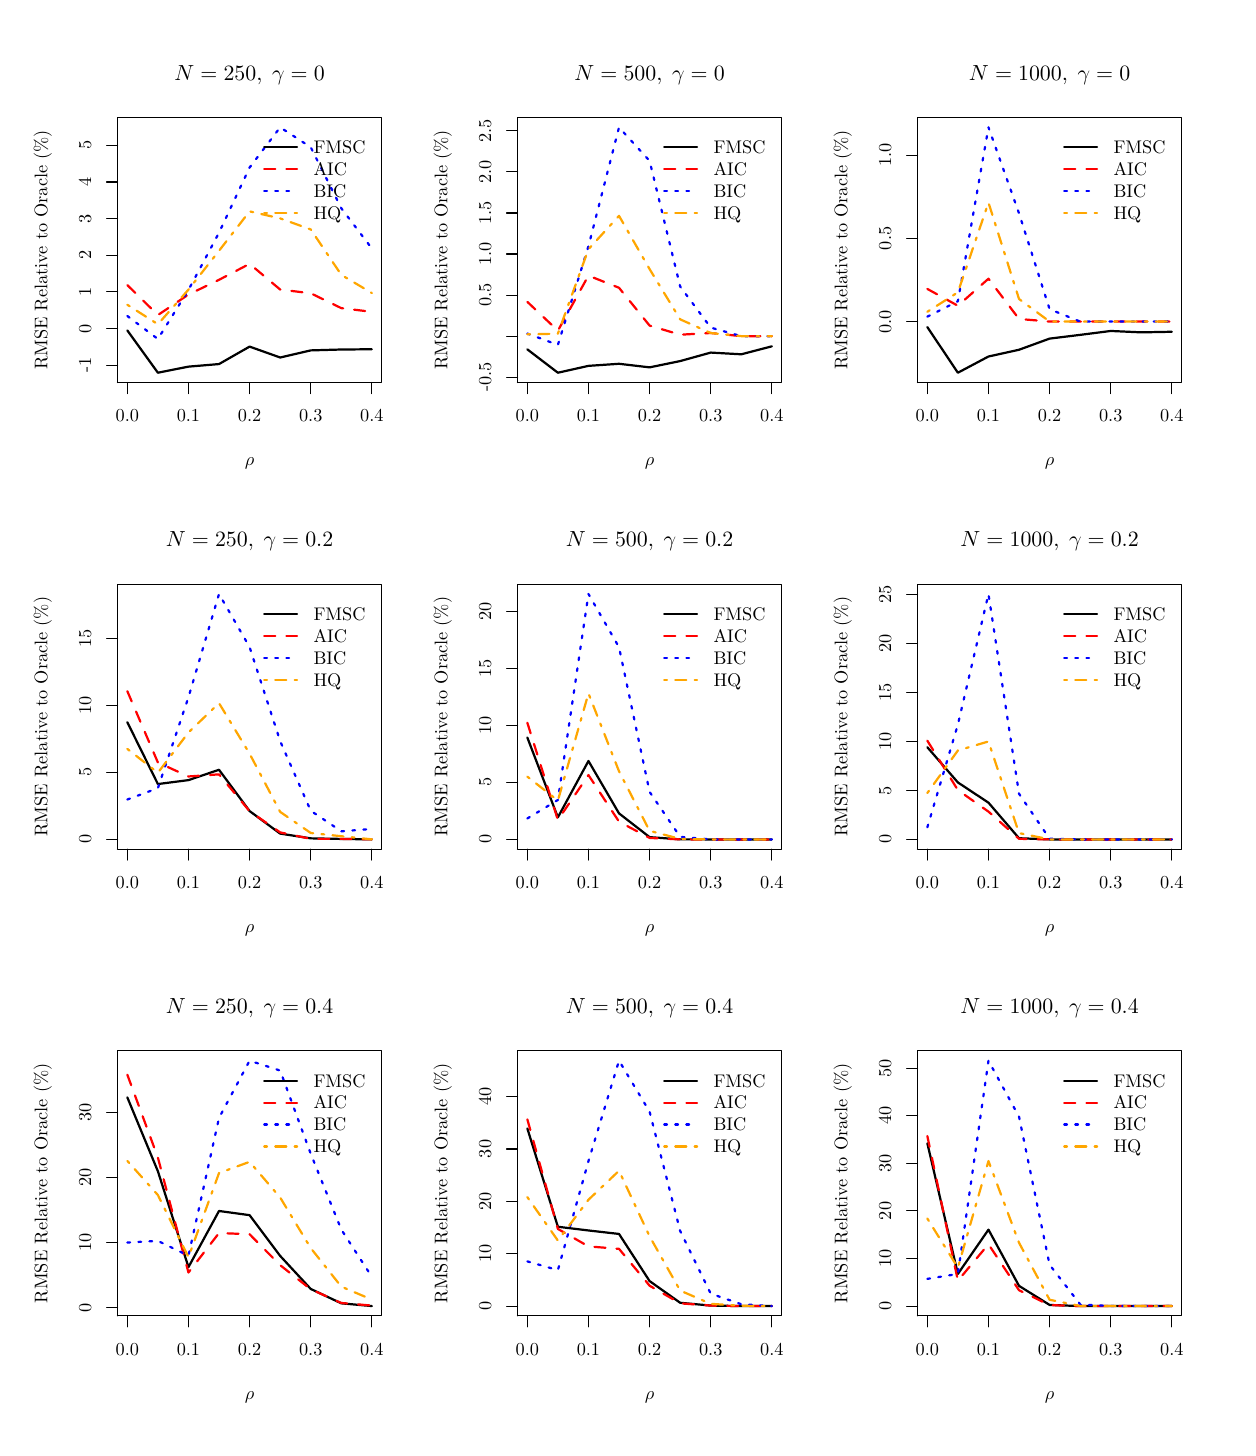
\begin{tikzpicture}[x=1pt,y=1pt]
\definecolor[named]{fillColor}{rgb}{1.00,1.00,1.00}
\path[use as bounding box,fill=fillColor,fill opacity=0.00] (0,0) rectangle (433.62,505.89);
\begin{scope}
\path[clip] ( 32.47,377.65) rectangle (127.91,473.42);
\definecolor[named]{drawColor}{rgb}{0.00,0.00,0.00}

\path[draw=drawColor,line width= 0.8pt,line join=round,line cap=round] ( 36.01,396.49) --
	( 47.05,381.20) --
	( 58.10,383.40) --
	( 69.14,384.33) --
	( 80.19,390.64) --
	( 91.24,386.70) --
	(102.28,389.27) --
	(113.33,389.59) --
	(124.37,389.68);
\end{scope}
\begin{scope}
\path[clip] (  0.00,  0.00) rectangle (433.62,505.89);
\definecolor[named]{drawColor}{rgb}{0.00,0.00,0.00}

\path[draw=drawColor,line width= 0.4pt,line join=round,line cap=round] ( 36.01,377.65) -- (124.37,377.65);

\path[draw=drawColor,line width= 0.4pt,line join=round,line cap=round] ( 36.01,377.65) -- ( 36.01,373.69);

\path[draw=drawColor,line width= 0.4pt,line join=round,line cap=round] ( 58.10,377.65) -- ( 58.10,373.69);

\path[draw=drawColor,line width= 0.4pt,line join=round,line cap=round] ( 80.19,377.65) -- ( 80.19,373.69);

\path[draw=drawColor,line width= 0.4pt,line join=round,line cap=round] (102.28,377.65) -- (102.28,373.69);

\path[draw=drawColor,line width= 0.4pt,line join=round,line cap=round] (124.37,377.65) -- (124.37,373.69);

\node[text=drawColor,anchor=base,inner sep=0pt, outer sep=0pt, scale=  0.66] at ( 36.01,363.40) {0.0};

\node[text=drawColor,anchor=base,inner sep=0pt, outer sep=0pt, scale=  0.66] at ( 58.10,363.40) {0.1};

\node[text=drawColor,anchor=base,inner sep=0pt, outer sep=0pt, scale=  0.66] at ( 80.19,363.40) {0.2};

\node[text=drawColor,anchor=base,inner sep=0pt, outer sep=0pt, scale=  0.66] at (102.28,363.40) {0.3};

\node[text=drawColor,anchor=base,inner sep=0pt, outer sep=0pt, scale=  0.66] at (124.37,363.40) {0.4};

\path[draw=drawColor,line width= 0.4pt,line join=round,line cap=round] ( 32.47,383.95) -- ( 32.47,463.36);

\path[draw=drawColor,line width= 0.4pt,line join=round,line cap=round] ( 32.47,383.95) -- ( 28.51,383.95);

\path[draw=drawColor,line width= 0.4pt,line join=round,line cap=round] ( 32.47,397.19) -- ( 28.51,397.19);

\path[draw=drawColor,line width= 0.4pt,line join=round,line cap=round] ( 32.47,410.42) -- ( 28.51,410.42);

\path[draw=drawColor,line width= 0.4pt,line join=round,line cap=round] ( 32.47,423.66) -- ( 28.51,423.66);

\path[draw=drawColor,line width= 0.4pt,line join=round,line cap=round] ( 32.47,436.89) -- ( 28.51,436.89);

\path[draw=drawColor,line width= 0.4pt,line join=round,line cap=round] ( 32.47,450.12) -- ( 28.51,450.12);

\path[draw=drawColor,line width= 0.4pt,line join=round,line cap=round] ( 32.47,463.36) -- ( 28.51,463.36);

\node[text=drawColor,rotate= 90.00,anchor=base,inner sep=0pt, outer sep=0pt, scale=  0.66] at ( 22.97,383.95) {-1};

\node[text=drawColor,rotate= 90.00,anchor=base,inner sep=0pt, outer sep=0pt, scale=  0.66] at ( 22.97,397.19) {0};

\node[text=drawColor,rotate= 90.00,anchor=base,inner sep=0pt, outer sep=0pt, scale=  0.66] at ( 22.97,410.42) {1};

\node[text=drawColor,rotate= 90.00,anchor=base,inner sep=0pt, outer sep=0pt, scale=  0.66] at ( 22.97,423.66) {2};

\node[text=drawColor,rotate= 90.00,anchor=base,inner sep=0pt, outer sep=0pt, scale=  0.66] at ( 22.97,436.89) {3};

\node[text=drawColor,rotate= 90.00,anchor=base,inner sep=0pt, outer sep=0pt, scale=  0.66] at ( 22.97,450.12) {4};

\node[text=drawColor,rotate= 90.00,anchor=base,inner sep=0pt, outer sep=0pt, scale=  0.66] at ( 22.97,463.36) {5};

\path[draw=drawColor,line width= 0.4pt,line join=round,line cap=round] ( 32.47,377.65) --
	(127.91,377.65) --
	(127.91,473.42) --
	( 32.47,473.42) --
	( 32.47,377.65);
\end{scope}
\begin{scope}
\path[clip] (  0.00,337.26) rectangle (144.54,505.89);
\definecolor[named]{drawColor}{rgb}{0.00,0.00,0.00}

\node[text=drawColor,anchor=base,inner sep=0pt, outer sep=0pt, scale=  0.79] at ( 80.19,486.92) {\bfseries $N=250, \;\gamma=0$};

\node[text=drawColor,anchor=base,inner sep=0pt, outer sep=0pt, scale=  0.66] at ( 80.19,347.56) {$\rho$};

\node[text=drawColor,rotate= 90.00,anchor=base,inner sep=0pt, outer sep=0pt, scale=  0.66] at (  7.13,425.53) {RMSE Relative to Oracle (\%)};
\end{scope}
\begin{scope}
\path[clip] ( 32.47,377.65) rectangle (127.91,473.42);
\definecolor[named]{drawColor}{rgb}{1.00,0.00,0.00}

\path[draw=drawColor,line width= 0.8pt,dash pattern=on 4pt off 4pt ,line join=round,line cap=round] ( 36.01,412.87) --
	( 47.05,402.05) --
	( 58.10,409.44) --
	( 69.14,414.77) --
	( 80.19,420.55) --
	( 91.24,411.26) --
	(102.28,409.91) --
	(113.33,404.54) --
	(124.37,403.21);
\definecolor[named]{drawColor}{rgb}{0.00,0.00,1.00}

\path[draw=drawColor,line width= 0.8pt,dash pattern=on 1pt off 3pt ,line join=round,line cap=round] ( 36.01,401.70) --
	( 47.05,393.38) --
	( 58.10,411.10) --
	( 69.14,431.79) --
	( 80.19,455.35) --
	( 91.24,469.87) --
	(102.28,462.69) --
	(113.33,440.62) --
	(124.37,426.10);
\definecolor[named]{drawColor}{rgb}{1.00,0.65,0.00}

\path[draw=drawColor,line width= 0.8pt,dash pattern=on 1pt off 3pt on 4pt off 3pt ,line join=round,line cap=round] ( 36.01,405.76) --
	( 47.05,398.72) --
	( 58.10,411.22) --
	( 69.14,425.26) --
	( 80.19,439.51) --
	( 91.24,436.97) --
	(102.28,432.98) --
	(113.33,416.56) --
	(124.37,409.99);
\definecolor[named]{drawColor}{rgb}{0.00,0.00,0.00}

\path[draw=drawColor,line width= 0.8pt,line join=round,line cap=round] ( 85.47,462.63) -- ( 97.35,462.63);
\definecolor[named]{drawColor}{rgb}{1.00,0.00,0.00}

\path[draw=drawColor,line width= 0.8pt,dash pattern=on 4pt off 4pt ,line join=round,line cap=round] ( 85.47,454.71) -- ( 97.35,454.71);
\definecolor[named]{drawColor}{rgb}{0.00,0.00,1.00}

\path[draw=drawColor,line width= 0.8pt,dash pattern=on 1pt off 3pt ,line join=round,line cap=round] ( 85.47,446.79) -- ( 97.35,446.79);
\definecolor[named]{drawColor}{rgb}{1.00,0.65,0.00}

\path[draw=drawColor,line width= 0.8pt,dash pattern=on 1pt off 3pt on 4pt off 3pt ,line join=round,line cap=round] ( 85.47,438.87) -- ( 97.35,438.87);
\definecolor[named]{drawColor}{rgb}{0.00,0.00,0.00}

\node[text=drawColor,anchor=base west,inner sep=0pt, outer sep=0pt, scale=  0.66] at (103.29,460.35) {FMSC};

\node[text=drawColor,anchor=base west,inner sep=0pt, outer sep=0pt, scale=  0.66] at (103.29,452.43) {AIC};

\node[text=drawColor,anchor=base west,inner sep=0pt, outer sep=0pt, scale=  0.66] at (103.29,444.51) {BIC};

\node[text=drawColor,anchor=base west,inner sep=0pt, outer sep=0pt, scale=  0.66] at (103.29,436.59) {HQ};
\end{scope}
\begin{scope}
\path[clip] (177.01,377.65) rectangle (272.45,473.42);
\definecolor[named]{drawColor}{rgb}{0.00,0.00,0.00}

\path[draw=drawColor,line width= 0.8pt,line join=round,line cap=round] (180.55,389.64) --
	(191.59,381.20) --
	(202.64,383.68) --
	(213.68,384.43) --
	(224.73,383.14) --
	(235.78,385.41) --
	(246.82,388.48) --
	(257.87,387.86) --
	(268.91,390.74);
\end{scope}
\begin{scope}
\path[clip] (  0.00,  0.00) rectangle (433.62,505.89);
\definecolor[named]{drawColor}{rgb}{0.00,0.00,0.00}

\path[draw=drawColor,line width= 0.4pt,line join=round,line cap=round] (180.55,377.65) -- (268.91,377.65);

\path[draw=drawColor,line width= 0.4pt,line join=round,line cap=round] (180.55,377.65) -- (180.55,373.69);

\path[draw=drawColor,line width= 0.4pt,line join=round,line cap=round] (202.64,377.65) -- (202.64,373.69);

\path[draw=drawColor,line width= 0.4pt,line join=round,line cap=round] (224.73,377.65) -- (224.73,373.69);

\path[draw=drawColor,line width= 0.4pt,line join=round,line cap=round] (246.82,377.65) -- (246.82,373.69);

\path[draw=drawColor,line width= 0.4pt,line join=round,line cap=round] (268.91,377.65) -- (268.91,373.69);

\node[text=drawColor,anchor=base,inner sep=0pt, outer sep=0pt, scale=  0.66] at (180.55,363.40) {0.0};

\node[text=drawColor,anchor=base,inner sep=0pt, outer sep=0pt, scale=  0.66] at (202.64,363.40) {0.1};

\node[text=drawColor,anchor=base,inner sep=0pt, outer sep=0pt, scale=  0.66] at (224.73,363.40) {0.2};

\node[text=drawColor,anchor=base,inner sep=0pt, outer sep=0pt, scale=  0.66] at (246.82,363.40) {0.3};

\node[text=drawColor,anchor=base,inner sep=0pt, outer sep=0pt, scale=  0.66] at (268.91,363.40) {0.4};

\path[draw=drawColor,line width= 0.4pt,line join=round,line cap=round] (177.01,379.57) -- (177.01,468.61);

\path[draw=drawColor,line width= 0.4pt,line join=round,line cap=round] (177.01,379.57) -- (173.05,379.57);

\path[draw=drawColor,line width= 0.4pt,line join=round,line cap=round] (177.01,394.41) -- (173.05,394.41);

\path[draw=drawColor,line width= 0.4pt,line join=round,line cap=round] (177.01,409.25) -- (173.05,409.25);

\path[draw=drawColor,line width= 0.4pt,line join=round,line cap=round] (177.01,424.09) -- (173.05,424.09);

\path[draw=drawColor,line width= 0.4pt,line join=round,line cap=round] (177.01,438.93) -- (173.05,438.93);

\path[draw=drawColor,line width= 0.4pt,line join=round,line cap=round] (177.01,453.77) -- (173.05,453.77);

\path[draw=drawColor,line width= 0.4pt,line join=round,line cap=round] (177.01,468.61) -- (173.05,468.61);

\node[text=drawColor,rotate= 90.00,anchor=base,inner sep=0pt, outer sep=0pt, scale=  0.66] at (167.51,379.57) {-0.5};

\node[text=drawColor,rotate= 90.00,anchor=base,inner sep=0pt, outer sep=0pt, scale=  0.66] at (167.51,409.25) {0.5};

\node[text=drawColor,rotate= 90.00,anchor=base,inner sep=0pt, outer sep=0pt, scale=  0.66] at (167.51,424.09) {1.0};

\node[text=drawColor,rotate= 90.00,anchor=base,inner sep=0pt, outer sep=0pt, scale=  0.66] at (167.51,438.93) {1.5};

\node[text=drawColor,rotate= 90.00,anchor=base,inner sep=0pt, outer sep=0pt, scale=  0.66] at (167.51,453.77) {2.0};

\node[text=drawColor,rotate= 90.00,anchor=base,inner sep=0pt, outer sep=0pt, scale=  0.66] at (167.51,468.61) {2.5};

\path[draw=drawColor,line width= 0.4pt,line join=round,line cap=round] (177.01,377.65) --
	(272.45,377.65) --
	(272.45,473.42) --
	(177.01,473.42) --
	(177.01,377.65);
\end{scope}
\begin{scope}
\path[clip] (144.54,337.26) rectangle (289.08,505.89);
\definecolor[named]{drawColor}{rgb}{0.00,0.00,0.00}

\node[text=drawColor,anchor=base,inner sep=0pt, outer sep=0pt, scale=  0.79] at (224.73,486.92) {\bfseries $N=500, \;\gamma=0$};

\node[text=drawColor,anchor=base,inner sep=0pt, outer sep=0pt, scale=  0.66] at (224.73,347.56) {$\rho$};

\node[text=drawColor,rotate= 90.00,anchor=base,inner sep=0pt, outer sep=0pt, scale=  0.66] at (151.67,425.53) {RMSE Relative to Oracle (\%)};
\end{scope}
\begin{scope}
\path[clip] (177.01,377.65) rectangle (272.45,473.42);
\definecolor[named]{drawColor}{rgb}{1.00,0.00,0.00}

\path[draw=drawColor,line width= 0.8pt,dash pattern=on 4pt off 4pt ,line join=round,line cap=round] (180.55,406.81) --
	(191.59,396.39) --
	(202.64,416.29) --
	(213.68,411.89) --
	(224.73,398.23) --
	(235.78,394.94) --
	(246.82,395.55) --
	(257.87,394.41) --
	(268.91,394.41);
\definecolor[named]{drawColor}{rgb}{0.00,0.00,1.00}

\path[draw=drawColor,line width= 0.8pt,dash pattern=on 1pt off 3pt ,line join=round,line cap=round] (180.55,395.37) --
	(191.59,391.25) --
	(202.64,426.93) --
	(213.68,469.87) --
	(224.73,457.75) --
	(235.78,412.35) --
	(246.82,397.50) --
	(257.87,394.41) --
	(268.91,394.41);
\definecolor[named]{drawColor}{rgb}{1.00,0.65,0.00}

\path[draw=drawColor,line width= 0.8pt,dash pattern=on 1pt off 3pt on 4pt off 3pt ,line join=round,line cap=round] (180.55,395.07) --
	(191.59,395.31) --
	(202.64,425.84) --
	(213.68,437.89) --
	(224.73,418.64) --
	(235.78,400.49) --
	(246.82,395.55) --
	(257.87,394.41) --
	(268.91,394.41);
\definecolor[named]{drawColor}{rgb}{0.00,0.00,0.00}

\path[draw=drawColor,line width= 0.8pt,line join=round,line cap=round] (230.01,462.63) -- (241.89,462.63);
\definecolor[named]{drawColor}{rgb}{1.00,0.00,0.00}

\path[draw=drawColor,line width= 0.8pt,dash pattern=on 4pt off 4pt ,line join=round,line cap=round] (230.01,454.71) -- (241.89,454.71);
\definecolor[named]{drawColor}{rgb}{0.00,0.00,1.00}

\path[draw=drawColor,line width= 0.8pt,dash pattern=on 1pt off 3pt ,line join=round,line cap=round] (230.01,446.79) -- (241.89,446.79);
\definecolor[named]{drawColor}{rgb}{1.00,0.65,0.00}

\path[draw=drawColor,line width= 0.8pt,dash pattern=on 1pt off 3pt on 4pt off 3pt ,line join=round,line cap=round] (230.01,438.87) -- (241.89,438.87);
\definecolor[named]{drawColor}{rgb}{0.00,0.00,0.00}

\node[text=drawColor,anchor=base west,inner sep=0pt, outer sep=0pt, scale=  0.66] at (247.83,460.35) {FMSC};

\node[text=drawColor,anchor=base west,inner sep=0pt, outer sep=0pt, scale=  0.66] at (247.83,452.43) {AIC};

\node[text=drawColor,anchor=base west,inner sep=0pt, outer sep=0pt, scale=  0.66] at (247.83,444.51) {BIC};

\node[text=drawColor,anchor=base west,inner sep=0pt, outer sep=0pt, scale=  0.66] at (247.83,436.59) {HQ};
\end{scope}
\begin{scope}
\path[clip] (321.55,377.65) rectangle (416.99,473.42);
\definecolor[named]{drawColor}{rgb}{0.00,0.00,0.00}

\path[draw=drawColor,line width= 0.8pt,line join=round,line cap=round] (325.09,397.69) --
	(336.13,381.20) --
	(347.18,387.06) --
	(358.22,389.50) --
	(369.27,393.53) --
	(380.32,394.88) --
	(391.36,396.29) --
	(402.41,395.79) --
	(413.45,396.00);
\end{scope}
\begin{scope}
\path[clip] (  0.00,  0.00) rectangle (433.62,505.89);
\definecolor[named]{drawColor}{rgb}{0.00,0.00,0.00}

\path[draw=drawColor,line width= 0.4pt,line join=round,line cap=round] (325.09,377.65) -- (413.45,377.65);

\path[draw=drawColor,line width= 0.4pt,line join=round,line cap=round] (325.09,377.65) -- (325.09,373.69);

\path[draw=drawColor,line width= 0.4pt,line join=round,line cap=round] (347.18,377.65) -- (347.18,373.69);

\path[draw=drawColor,line width= 0.4pt,line join=round,line cap=round] (369.27,377.65) -- (369.27,373.69);

\path[draw=drawColor,line width= 0.4pt,line join=round,line cap=round] (391.36,377.65) -- (391.36,373.69);

\path[draw=drawColor,line width= 0.4pt,line join=round,line cap=round] (413.45,377.65) -- (413.45,373.69);

\node[text=drawColor,anchor=base,inner sep=0pt, outer sep=0pt, scale=  0.66] at (325.09,363.40) {0.0};

\node[text=drawColor,anchor=base,inner sep=0pt, outer sep=0pt, scale=  0.66] at (347.18,363.40) {0.1};

\node[text=drawColor,anchor=base,inner sep=0pt, outer sep=0pt, scale=  0.66] at (369.27,363.40) {0.2};

\node[text=drawColor,anchor=base,inner sep=0pt, outer sep=0pt, scale=  0.66] at (391.36,363.40) {0.3};

\node[text=drawColor,anchor=base,inner sep=0pt, outer sep=0pt, scale=  0.66] at (413.45,363.40) {0.4};

\path[draw=drawColor,line width= 0.4pt,line join=round,line cap=round] (321.55,399.69) -- (321.55,459.81);

\path[draw=drawColor,line width= 0.4pt,line join=round,line cap=round] (321.55,399.69) -- (317.59,399.69);

\path[draw=drawColor,line width= 0.4pt,line join=round,line cap=round] (321.55,429.75) -- (317.59,429.75);

\path[draw=drawColor,line width= 0.4pt,line join=round,line cap=round] (321.55,459.81) -- (317.59,459.81);

\node[text=drawColor,rotate= 90.00,anchor=base,inner sep=0pt, outer sep=0pt, scale=  0.66] at (312.05,399.69) {0.0};

\node[text=drawColor,rotate= 90.00,anchor=base,inner sep=0pt, outer sep=0pt, scale=  0.66] at (312.05,429.75) {0.5};

\node[text=drawColor,rotate= 90.00,anchor=base,inner sep=0pt, outer sep=0pt, scale=  0.66] at (312.05,459.81) {1.0};

\path[draw=drawColor,line width= 0.4pt,line join=round,line cap=round] (321.55,377.65) --
	(416.99,377.65) --
	(416.99,473.42) --
	(321.55,473.42) --
	(321.55,377.65);
\end{scope}
\begin{scope}
\path[clip] (289.08,337.26) rectangle (433.62,505.89);
\definecolor[named]{drawColor}{rgb}{0.00,0.00,0.00}

\node[text=drawColor,anchor=base,inner sep=0pt, outer sep=0pt, scale=  0.79] at (369.27,486.92) {\bfseries $N=1000, \;\gamma=0$};

\node[text=drawColor,anchor=base,inner sep=0pt, outer sep=0pt, scale=  0.66] at (369.27,347.56) {$\rho$};

\node[text=drawColor,rotate= 90.00,anchor=base,inner sep=0pt, outer sep=0pt, scale=  0.66] at (296.21,425.53) {RMSE Relative to Oracle (\%)};
\end{scope}
\begin{scope}
\path[clip] (321.55,377.65) rectangle (416.99,473.42);
\definecolor[named]{drawColor}{rgb}{1.00,0.00,0.00}

\path[draw=drawColor,line width= 0.8pt,dash pattern=on 4pt off 4pt ,line join=round,line cap=round] (325.09,411.48) --
	(336.13,405.40) --
	(347.18,415.17) --
	(358.22,400.63) --
	(369.27,399.69) --
	(380.32,399.69) --
	(391.36,399.69) --
	(402.41,399.69) --
	(413.45,399.69);
\definecolor[named]{drawColor}{rgb}{0.00,0.00,1.00}

\path[draw=drawColor,line width= 0.8pt,dash pattern=on 1pt off 3pt ,line join=round,line cap=round] (325.09,401.45) --
	(336.13,407.03) --
	(347.18,469.87) --
	(358.22,438.81) --
	(369.27,404.16) --
	(380.32,399.69) --
	(391.36,399.69) --
	(402.41,399.69) --
	(413.45,399.69);
\definecolor[named]{drawColor}{rgb}{1.00,0.65,0.00}

\path[draw=drawColor,line width= 0.8pt,dash pattern=on 1pt off 3pt on 4pt off 3pt ,line join=round,line cap=round] (325.09,403.22) --
	(336.13,410.25) --
	(347.18,442.68) --
	(358.22,407.84) --
	(369.27,399.69) --
	(380.32,399.69) --
	(391.36,399.69) --
	(402.41,399.69) --
	(413.45,399.69);
\definecolor[named]{drawColor}{rgb}{0.00,0.00,0.00}

\path[draw=drawColor,line width= 0.8pt,line join=round,line cap=round] (374.55,462.63) -- (386.43,462.63);
\definecolor[named]{drawColor}{rgb}{1.00,0.00,0.00}

\path[draw=drawColor,line width= 0.8pt,dash pattern=on 4pt off 4pt ,line join=round,line cap=round] (374.55,454.71) -- (386.43,454.71);
\definecolor[named]{drawColor}{rgb}{0.00,0.00,1.00}

\path[draw=drawColor,line width= 0.8pt,dash pattern=on 1pt off 3pt ,line join=round,line cap=round] (374.55,446.79) -- (386.43,446.79);
\definecolor[named]{drawColor}{rgb}{1.00,0.65,0.00}

\path[draw=drawColor,line width= 0.8pt,dash pattern=on 1pt off 3pt on 4pt off 3pt ,line join=round,line cap=round] (374.55,438.87) -- (386.43,438.87);
\definecolor[named]{drawColor}{rgb}{0.00,0.00,0.00}

\node[text=drawColor,anchor=base west,inner sep=0pt, outer sep=0pt, scale=  0.66] at (392.37,460.35) {FMSC};

\node[text=drawColor,anchor=base west,inner sep=0pt, outer sep=0pt, scale=  0.66] at (392.37,452.43) {AIC};

\node[text=drawColor,anchor=base west,inner sep=0pt, outer sep=0pt, scale=  0.66] at (392.37,444.51) {BIC};

\node[text=drawColor,anchor=base west,inner sep=0pt, outer sep=0pt, scale=  0.66] at (392.37,436.59) {HQ};
\end{scope}
\begin{scope}
\path[clip] ( 32.47,209.02) rectangle (127.91,304.79);
\definecolor[named]{drawColor}{rgb}{0.00,0.00,0.00}

\path[draw=drawColor,line width= 0.8pt,line join=round,line cap=round] ( 36.01,254.91) --
	( 47.05,232.57) --
	( 58.10,233.99) --
	( 69.14,237.73) --
	( 80.19,222.81) --
	( 91.24,214.66) --
	(102.28,212.95) --
	(113.33,212.74) --
	(124.37,212.57);
\end{scope}
\begin{scope}
\path[clip] (  0.00,  0.00) rectangle (433.62,505.89);
\definecolor[named]{drawColor}{rgb}{0.00,0.00,0.00}

\path[draw=drawColor,line width= 0.4pt,line join=round,line cap=round] ( 36.01,209.02) -- (124.37,209.02);

\path[draw=drawColor,line width= 0.4pt,line join=round,line cap=round] ( 36.01,209.02) -- ( 36.01,205.06);

\path[draw=drawColor,line width= 0.4pt,line join=round,line cap=round] ( 58.10,209.02) -- ( 58.10,205.06);

\path[draw=drawColor,line width= 0.4pt,line join=round,line cap=round] ( 80.19,209.02) -- ( 80.19,205.06);

\path[draw=drawColor,line width= 0.4pt,line join=round,line cap=round] (102.28,209.02) -- (102.28,205.06);

\path[draw=drawColor,line width= 0.4pt,line join=round,line cap=round] (124.37,209.02) -- (124.37,205.06);

\node[text=drawColor,anchor=base,inner sep=0pt, outer sep=0pt, scale=  0.66] at ( 36.01,194.77) {0.0};

\node[text=drawColor,anchor=base,inner sep=0pt, outer sep=0pt, scale=  0.66] at ( 58.10,194.77) {0.1};

\node[text=drawColor,anchor=base,inner sep=0pt, outer sep=0pt, scale=  0.66] at ( 80.19,194.77) {0.2};

\node[text=drawColor,anchor=base,inner sep=0pt, outer sep=0pt, scale=  0.66] at (102.28,194.77) {0.3};

\node[text=drawColor,anchor=base,inner sep=0pt, outer sep=0pt, scale=  0.66] at (124.37,194.77) {0.4};

\path[draw=drawColor,line width= 0.4pt,line join=round,line cap=round] ( 32.47,212.59) -- ( 32.47,285.16);

\path[draw=drawColor,line width= 0.4pt,line join=round,line cap=round] ( 32.47,212.59) -- ( 28.51,212.59);

\path[draw=drawColor,line width= 0.4pt,line join=round,line cap=round] ( 32.47,236.78) -- ( 28.51,236.78);

\path[draw=drawColor,line width= 0.4pt,line join=round,line cap=round] ( 32.47,260.97) -- ( 28.51,260.97);

\path[draw=drawColor,line width= 0.4pt,line join=round,line cap=round] ( 32.47,285.16) -- ( 28.51,285.16);

\node[text=drawColor,rotate= 90.00,anchor=base,inner sep=0pt, outer sep=0pt, scale=  0.66] at ( 22.97,212.59) {0};

\node[text=drawColor,rotate= 90.00,anchor=base,inner sep=0pt, outer sep=0pt, scale=  0.66] at ( 22.97,236.78) {5};

\node[text=drawColor,rotate= 90.00,anchor=base,inner sep=0pt, outer sep=0pt, scale=  0.66] at ( 22.97,260.97) {10};

\node[text=drawColor,rotate= 90.00,anchor=base,inner sep=0pt, outer sep=0pt, scale=  0.66] at ( 22.97,285.16) {15};

\path[draw=drawColor,line width= 0.4pt,line join=round,line cap=round] ( 32.47,209.02) --
	(127.91,209.02) --
	(127.91,304.79) --
	( 32.47,304.79) --
	( 32.47,209.02);
\end{scope}
\begin{scope}
\path[clip] (  0.00,168.63) rectangle (144.54,337.26);
\definecolor[named]{drawColor}{rgb}{0.00,0.00,0.00}

\node[text=drawColor,anchor=base,inner sep=0pt, outer sep=0pt, scale=  0.79] at ( 80.19,318.29) {\bfseries $N=250, \;\gamma=0.2$};

\node[text=drawColor,anchor=base,inner sep=0pt, outer sep=0pt, scale=  0.66] at ( 80.19,178.93) {$\rho$};

\node[text=drawColor,rotate= 90.00,anchor=base,inner sep=0pt, outer sep=0pt, scale=  0.66] at (  7.13,256.90) {RMSE Relative to Oracle (\%)};
\end{scope}
\begin{scope}
\path[clip] ( 32.47,209.02) rectangle (127.91,304.79);
\definecolor[named]{drawColor}{rgb}{1.00,0.00,0.00}

\path[draw=drawColor,line width= 0.8pt,dash pattern=on 4pt off 4pt ,line join=round,line cap=round] ( 36.01,266.12) --
	( 47.05,240.36) --
	( 58.10,235.31) --
	( 69.14,236.07) --
	( 80.19,222.76) --
	( 91.24,215.10) --
	(102.28,212.76) --
	(113.33,212.76) --
	(124.37,212.59);
\definecolor[named]{drawColor}{rgb}{0.00,0.00,1.00}

\path[draw=drawColor,line width= 0.8pt,dash pattern=on 1pt off 3pt ,line join=round,line cap=round] ( 36.01,226.98) --
	( 47.05,231.09) --
	( 58.10,263.94) --
	( 69.14,301.24) --
	( 80.19,282.08) --
	( 91.24,248.07) --
	(102.28,222.93) --
	(113.33,215.49) --
	(124.37,216.35);
\definecolor[named]{drawColor}{rgb}{1.00,0.65,0.00}

\path[draw=drawColor,line width= 0.8pt,dash pattern=on 1pt off 3pt on 4pt off 3pt ,line join=round,line cap=round] ( 36.01,245.26) --
	( 47.05,236.64) --
	( 58.10,251.20) --
	( 69.14,261.81) --
	( 80.19,243.54) --
	( 91.24,222.52) --
	(102.28,214.89) --
	(113.33,213.72) --
	(124.37,212.59);
\definecolor[named]{drawColor}{rgb}{0.00,0.00,0.00}

\path[draw=drawColor,line width= 0.8pt,line join=round,line cap=round] ( 85.47,294.00) -- ( 97.35,294.00);
\definecolor[named]{drawColor}{rgb}{1.00,0.00,0.00}

\path[draw=drawColor,line width= 0.8pt,dash pattern=on 4pt off 4pt ,line join=round,line cap=round] ( 85.47,286.08) -- ( 97.35,286.08);
\definecolor[named]{drawColor}{rgb}{0.00,0.00,1.00}

\path[draw=drawColor,line width= 0.8pt,dash pattern=on 1pt off 3pt ,line join=round,line cap=round] ( 85.47,278.16) -- ( 97.35,278.16);
\definecolor[named]{drawColor}{rgb}{1.00,0.65,0.00}

\path[draw=drawColor,line width= 0.8pt,dash pattern=on 1pt off 3pt on 4pt off 3pt ,line join=round,line cap=round] ( 85.47,270.24) -- ( 97.35,270.24);
\definecolor[named]{drawColor}{rgb}{0.00,0.00,0.00}

\node[text=drawColor,anchor=base west,inner sep=0pt, outer sep=0pt, scale=  0.66] at (103.29,291.72) {FMSC};

\node[text=drawColor,anchor=base west,inner sep=0pt, outer sep=0pt, scale=  0.66] at (103.29,283.80) {AIC};

\node[text=drawColor,anchor=base west,inner sep=0pt, outer sep=0pt, scale=  0.66] at (103.29,275.88) {BIC};

\node[text=drawColor,anchor=base west,inner sep=0pt, outer sep=0pt, scale=  0.66] at (103.29,267.96) {HQ};
\end{scope}
\begin{scope}
\path[clip] (177.01,209.02) rectangle (272.45,304.79);
\definecolor[named]{drawColor}{rgb}{0.00,0.00,0.00}

\path[draw=drawColor,line width= 0.8pt,line join=round,line cap=round] (180.55,249.38) --
	(191.59,220.54) --
	(202.64,240.91) --
	(213.68,221.97) --
	(224.73,213.39) --
	(235.78,212.58) --
	(246.82,212.57) --
	(257.87,212.57) --
	(268.91,212.57);
\end{scope}
\begin{scope}
\path[clip] (  0.00,  0.00) rectangle (433.62,505.89);
\definecolor[named]{drawColor}{rgb}{0.00,0.00,0.00}

\path[draw=drawColor,line width= 0.4pt,line join=round,line cap=round] (180.55,209.02) -- (268.91,209.02);

\path[draw=drawColor,line width= 0.4pt,line join=round,line cap=round] (180.55,209.02) -- (180.55,205.06);

\path[draw=drawColor,line width= 0.4pt,line join=round,line cap=round] (202.64,209.02) -- (202.64,205.06);

\path[draw=drawColor,line width= 0.4pt,line join=round,line cap=round] (224.73,209.02) -- (224.73,205.06);

\path[draw=drawColor,line width= 0.4pt,line join=round,line cap=round] (246.82,209.02) -- (246.82,205.06);

\path[draw=drawColor,line width= 0.4pt,line join=round,line cap=round] (268.91,209.02) -- (268.91,205.06);

\node[text=drawColor,anchor=base,inner sep=0pt, outer sep=0pt, scale=  0.66] at (180.55,194.77) {0.0};

\node[text=drawColor,anchor=base,inner sep=0pt, outer sep=0pt, scale=  0.66] at (202.64,194.77) {0.1};

\node[text=drawColor,anchor=base,inner sep=0pt, outer sep=0pt, scale=  0.66] at (224.73,194.77) {0.2};

\node[text=drawColor,anchor=base,inner sep=0pt, outer sep=0pt, scale=  0.66] at (246.82,194.77) {0.3};

\node[text=drawColor,anchor=base,inner sep=0pt, outer sep=0pt, scale=  0.66] at (268.91,194.77) {0.4};

\path[draw=drawColor,line width= 0.4pt,line join=round,line cap=round] (177.01,212.57) -- (177.01,295.01);

\path[draw=drawColor,line width= 0.4pt,line join=round,line cap=round] (177.01,212.57) -- (173.05,212.57);

\path[draw=drawColor,line width= 0.4pt,line join=round,line cap=round] (177.01,233.18) -- (173.05,233.18);

\path[draw=drawColor,line width= 0.4pt,line join=round,line cap=round] (177.01,253.79) -- (173.05,253.79);

\path[draw=drawColor,line width= 0.4pt,line join=round,line cap=round] (177.01,274.40) -- (173.05,274.40);

\path[draw=drawColor,line width= 0.4pt,line join=round,line cap=round] (177.01,295.01) -- (173.05,295.01);

\node[text=drawColor,rotate= 90.00,anchor=base,inner sep=0pt, outer sep=0pt, scale=  0.66] at (167.51,212.57) {0};

\node[text=drawColor,rotate= 90.00,anchor=base,inner sep=0pt, outer sep=0pt, scale=  0.66] at (167.51,233.18) {5};

\node[text=drawColor,rotate= 90.00,anchor=base,inner sep=0pt, outer sep=0pt, scale=  0.66] at (167.51,253.79) {10};

\node[text=drawColor,rotate= 90.00,anchor=base,inner sep=0pt, outer sep=0pt, scale=  0.66] at (167.51,274.40) {15};

\node[text=drawColor,rotate= 90.00,anchor=base,inner sep=0pt, outer sep=0pt, scale=  0.66] at (167.51,295.01) {20};

\path[draw=drawColor,line width= 0.4pt,line join=round,line cap=round] (177.01,209.02) --
	(272.45,209.02) --
	(272.45,304.79) --
	(177.01,304.79) --
	(177.01,209.02);
\end{scope}
\begin{scope}
\path[clip] (144.54,168.63) rectangle (289.08,337.26);
\definecolor[named]{drawColor}{rgb}{0.00,0.00,0.00}

\node[text=drawColor,anchor=base,inner sep=0pt, outer sep=0pt, scale=  0.79] at (224.73,318.29) {\bfseries $N=500, \;\gamma=0.2$};

\node[text=drawColor,anchor=base,inner sep=0pt, outer sep=0pt, scale=  0.66] at (224.73,178.93) {$\rho$};

\node[text=drawColor,rotate= 90.00,anchor=base,inner sep=0pt, outer sep=0pt, scale=  0.66] at (151.67,256.90) {RMSE Relative to Oracle (\%)};
\end{scope}
\begin{scope}
\path[clip] (177.01,209.02) rectangle (272.45,304.79);
\definecolor[named]{drawColor}{rgb}{1.00,0.00,0.00}

\path[draw=drawColor,line width= 0.8pt,dash pattern=on 4pt off 4pt ,line join=round,line cap=round] (180.55,254.72) --
	(191.59,219.59) --
	(202.64,235.82) --
	(213.68,218.97) --
	(224.73,213.10) --
	(235.78,212.57) --
	(246.82,212.57) --
	(257.87,212.57) --
	(268.91,212.57);
\definecolor[named]{drawColor}{rgb}{0.00,0.00,1.00}

\path[draw=drawColor,line width= 0.8pt,dash pattern=on 1pt off 3pt ,line join=round,line cap=round] (180.55,220.13) --
	(191.59,226.82) --
	(202.64,301.24) --
	(213.68,282.01) --
	(224.73,229.74) --
	(235.78,213.49) --
	(246.82,212.57) --
	(257.87,212.57) --
	(268.91,212.57);
\definecolor[named]{drawColor}{rgb}{1.00,0.65,0.00}

\path[draw=drawColor,line width= 0.8pt,dash pattern=on 1pt off 3pt on 4pt off 3pt ,line join=round,line cap=round] (180.55,235.25) --
	(191.59,226.61) --
	(202.64,265.34) --
	(213.68,237.18) --
	(224.73,215.66) --
	(235.78,212.74) --
	(246.82,212.57) --
	(257.87,212.57) --
	(268.91,212.57);
\definecolor[named]{drawColor}{rgb}{0.00,0.00,0.00}

\path[draw=drawColor,line width= 0.8pt,line join=round,line cap=round] (230.01,294.00) -- (241.89,294.00);
\definecolor[named]{drawColor}{rgb}{1.00,0.00,0.00}

\path[draw=drawColor,line width= 0.8pt,dash pattern=on 4pt off 4pt ,line join=round,line cap=round] (230.01,286.08) -- (241.89,286.08);
\definecolor[named]{drawColor}{rgb}{0.00,0.00,1.00}

\path[draw=drawColor,line width= 0.8pt,dash pattern=on 1pt off 3pt ,line join=round,line cap=round] (230.01,278.16) -- (241.89,278.16);
\definecolor[named]{drawColor}{rgb}{1.00,0.65,0.00}

\path[draw=drawColor,line width= 0.8pt,dash pattern=on 1pt off 3pt on 4pt off 3pt ,line join=round,line cap=round] (230.01,270.24) -- (241.89,270.24);
\definecolor[named]{drawColor}{rgb}{0.00,0.00,0.00}

\node[text=drawColor,anchor=base west,inner sep=0pt, outer sep=0pt, scale=  0.66] at (247.83,291.72) {FMSC};

\node[text=drawColor,anchor=base west,inner sep=0pt, outer sep=0pt, scale=  0.66] at (247.83,283.80) {AIC};

\node[text=drawColor,anchor=base west,inner sep=0pt, outer sep=0pt, scale=  0.66] at (247.83,275.88) {BIC};

\node[text=drawColor,anchor=base west,inner sep=0pt, outer sep=0pt, scale=  0.66] at (247.83,267.96) {HQ};
\end{scope}
\begin{scope}
\path[clip] (321.55,209.02) rectangle (416.99,304.79);
\definecolor[named]{drawColor}{rgb}{0.00,0.00,0.00}

\path[draw=drawColor,line width= 0.8pt,line join=round,line cap=round] (325.09,245.87) --
	(336.13,233.15) --
	(347.18,225.84) --
	(358.22,212.99) --
	(369.27,212.57) --
	(380.32,212.57) --
	(391.36,212.57) --
	(402.41,212.57) --
	(413.45,212.57);
\end{scope}
\begin{scope}
\path[clip] (  0.00,  0.00) rectangle (433.62,505.89);
\definecolor[named]{drawColor}{rgb}{0.00,0.00,0.00}

\path[draw=drawColor,line width= 0.4pt,line join=round,line cap=round] (325.09,209.02) -- (413.45,209.02);

\path[draw=drawColor,line width= 0.4pt,line join=round,line cap=round] (325.09,209.02) -- (325.09,205.06);

\path[draw=drawColor,line width= 0.4pt,line join=round,line cap=round] (347.18,209.02) -- (347.18,205.06);

\path[draw=drawColor,line width= 0.4pt,line join=round,line cap=round] (369.27,209.02) -- (369.27,205.06);

\path[draw=drawColor,line width= 0.4pt,line join=round,line cap=round] (391.36,209.02) -- (391.36,205.06);

\path[draw=drawColor,line width= 0.4pt,line join=round,line cap=round] (413.45,209.02) -- (413.45,205.06);

\node[text=drawColor,anchor=base,inner sep=0pt, outer sep=0pt, scale=  0.66] at (325.09,194.77) {0.0};

\node[text=drawColor,anchor=base,inner sep=0pt, outer sep=0pt, scale=  0.66] at (347.18,194.77) {0.1};

\node[text=drawColor,anchor=base,inner sep=0pt, outer sep=0pt, scale=  0.66] at (369.27,194.77) {0.2};

\node[text=drawColor,anchor=base,inner sep=0pt, outer sep=0pt, scale=  0.66] at (391.36,194.77) {0.3};

\node[text=drawColor,anchor=base,inner sep=0pt, outer sep=0pt, scale=  0.66] at (413.45,194.77) {0.4};

\path[draw=drawColor,line width= 0.4pt,line join=round,line cap=round] (321.55,212.57) -- (321.55,301.05);

\path[draw=drawColor,line width= 0.4pt,line join=round,line cap=round] (321.55,212.57) -- (317.59,212.57);

\path[draw=drawColor,line width= 0.4pt,line join=round,line cap=round] (321.55,230.26) -- (317.59,230.26);

\path[draw=drawColor,line width= 0.4pt,line join=round,line cap=round] (321.55,247.96) -- (317.59,247.96);

\path[draw=drawColor,line width= 0.4pt,line join=round,line cap=round] (321.55,265.66) -- (317.59,265.66);

\path[draw=drawColor,line width= 0.4pt,line join=round,line cap=round] (321.55,283.35) -- (317.59,283.35);

\path[draw=drawColor,line width= 0.4pt,line join=round,line cap=round] (321.55,301.05) -- (317.59,301.05);

\node[text=drawColor,rotate= 90.00,anchor=base,inner sep=0pt, outer sep=0pt, scale=  0.66] at (312.05,212.57) {0};

\node[text=drawColor,rotate= 90.00,anchor=base,inner sep=0pt, outer sep=0pt, scale=  0.66] at (312.05,230.26) {5};

\node[text=drawColor,rotate= 90.00,anchor=base,inner sep=0pt, outer sep=0pt, scale=  0.66] at (312.05,247.96) {10};

\node[text=drawColor,rotate= 90.00,anchor=base,inner sep=0pt, outer sep=0pt, scale=  0.66] at (312.05,265.66) {15};

\node[text=drawColor,rotate= 90.00,anchor=base,inner sep=0pt, outer sep=0pt, scale=  0.66] at (312.05,283.35) {20};

\node[text=drawColor,rotate= 90.00,anchor=base,inner sep=0pt, outer sep=0pt, scale=  0.66] at (312.05,301.05) {25};

\path[draw=drawColor,line width= 0.4pt,line join=round,line cap=round] (321.55,209.02) --
	(416.99,209.02) --
	(416.99,304.79) --
	(321.55,304.79) --
	(321.55,209.02);
\end{scope}
\begin{scope}
\path[clip] (289.08,168.63) rectangle (433.62,337.26);
\definecolor[named]{drawColor}{rgb}{0.00,0.00,0.00}

\node[text=drawColor,anchor=base,inner sep=0pt, outer sep=0pt, scale=  0.79] at (369.27,318.29) {\bfseries $N=1000, \;\gamma=0.2$};

\node[text=drawColor,anchor=base,inner sep=0pt, outer sep=0pt, scale=  0.66] at (369.27,178.93) {$\rho$};

\node[text=drawColor,rotate= 90.00,anchor=base,inner sep=0pt, outer sep=0pt, scale=  0.66] at (296.21,256.90) {RMSE Relative to Oracle (\%)};
\end{scope}
\begin{scope}
\path[clip] (321.55,209.02) rectangle (416.99,304.79);
\definecolor[named]{drawColor}{rgb}{1.00,0.00,0.00}

\path[draw=drawColor,line width= 0.8pt,dash pattern=on 4pt off 4pt ,line join=round,line cap=round] (325.09,248.24) --
	(336.13,230.38) --
	(347.18,222.61) --
	(358.22,212.78) --
	(369.27,212.57) --
	(380.32,212.57) --
	(391.36,212.57) --
	(402.41,212.57) --
	(413.45,212.57);
\definecolor[named]{drawColor}{rgb}{0.00,0.00,1.00}

\path[draw=drawColor,line width= 0.8pt,dash pattern=on 1pt off 3pt ,line join=round,line cap=round] (325.09,216.95) --
	(336.13,254.09) --
	(347.18,301.24) --
	(358.22,229.07) --
	(369.27,212.80) --
	(380.32,212.57) --
	(391.36,212.57) --
	(402.41,212.57) --
	(413.45,212.57);
\definecolor[named]{drawColor}{rgb}{1.00,0.65,0.00}

\path[draw=drawColor,line width= 0.8pt,dash pattern=on 1pt off 3pt on 4pt off 3pt ,line join=round,line cap=round] (325.09,229.32) --
	(336.13,244.70) --
	(347.18,247.96) --
	(358.22,214.85) --
	(369.27,212.57) --
	(380.32,212.57) --
	(391.36,212.57) --
	(402.41,212.57) --
	(413.45,212.57);
\definecolor[named]{drawColor}{rgb}{0.00,0.00,0.00}

\path[draw=drawColor,line width= 0.8pt,line join=round,line cap=round] (374.55,294.00) -- (386.43,294.00);
\definecolor[named]{drawColor}{rgb}{1.00,0.00,0.00}

\path[draw=drawColor,line width= 0.8pt,dash pattern=on 4pt off 4pt ,line join=round,line cap=round] (374.55,286.08) -- (386.43,286.08);
\definecolor[named]{drawColor}{rgb}{0.00,0.00,1.00}

\path[draw=drawColor,line width= 0.8pt,dash pattern=on 1pt off 3pt ,line join=round,line cap=round] (374.55,278.16) -- (386.43,278.16);
\definecolor[named]{drawColor}{rgb}{1.00,0.65,0.00}

\path[draw=drawColor,line width= 0.8pt,dash pattern=on 1pt off 3pt on 4pt off 3pt ,line join=round,line cap=round] (374.55,270.24) -- (386.43,270.24);
\definecolor[named]{drawColor}{rgb}{0.00,0.00,0.00}

\node[text=drawColor,anchor=base west,inner sep=0pt, outer sep=0pt, scale=  0.66] at (392.37,291.72) {FMSC};

\node[text=drawColor,anchor=base west,inner sep=0pt, outer sep=0pt, scale=  0.66] at (392.37,283.80) {AIC};

\node[text=drawColor,anchor=base west,inner sep=0pt, outer sep=0pt, scale=  0.66] at (392.37,275.88) {BIC};

\node[text=drawColor,anchor=base west,inner sep=0pt, outer sep=0pt, scale=  0.66] at (392.37,267.96) {HQ};
\end{scope}
\begin{scope}
\path[clip] ( 32.47, 40.39) rectangle (127.91,136.16);
\definecolor[named]{drawColor}{rgb}{0.00,0.00,0.00}

\path[draw=drawColor,line width= 0.8pt,line join=round,line cap=round] ( 36.01,119.35) --
	( 47.05, 92.66) --
	( 58.10, 58.02) --
	( 69.14, 78.30) --
	( 80.19, 76.79) --
	( 91.24, 62.06) --
	(102.28, 50.13) --
	(113.33, 44.93) --
	(124.37, 43.94);
\end{scope}
\begin{scope}
\path[clip] (  0.00,  0.00) rectangle (433.62,505.89);
\definecolor[named]{drawColor}{rgb}{0.00,0.00,0.00}

\path[draw=drawColor,line width= 0.4pt,line join=round,line cap=round] ( 36.01, 40.39) -- (124.37, 40.39);

\path[draw=drawColor,line width= 0.4pt,line join=round,line cap=round] ( 36.01, 40.39) -- ( 36.01, 36.43);

\path[draw=drawColor,line width= 0.4pt,line join=round,line cap=round] ( 58.10, 40.39) -- ( 58.10, 36.43);

\path[draw=drawColor,line width= 0.4pt,line join=round,line cap=round] ( 80.19, 40.39) -- ( 80.19, 36.43);

\path[draw=drawColor,line width= 0.4pt,line join=round,line cap=round] (102.28, 40.39) -- (102.28, 36.43);

\path[draw=drawColor,line width= 0.4pt,line join=round,line cap=round] (124.37, 40.39) -- (124.37, 36.43);

\node[text=drawColor,anchor=base,inner sep=0pt, outer sep=0pt, scale=  0.66] at ( 36.01, 26.14) {0.0};

\node[text=drawColor,anchor=base,inner sep=0pt, outer sep=0pt, scale=  0.66] at ( 58.10, 26.14) {0.1};

\node[text=drawColor,anchor=base,inner sep=0pt, outer sep=0pt, scale=  0.66] at ( 80.19, 26.14) {0.2};

\node[text=drawColor,anchor=base,inner sep=0pt, outer sep=0pt, scale=  0.66] at (102.28, 26.14) {0.3};

\node[text=drawColor,anchor=base,inner sep=0pt, outer sep=0pt, scale=  0.66] at (124.37, 26.14) {0.4};

\path[draw=drawColor,line width= 0.4pt,line join=round,line cap=round] ( 32.47, 43.44) -- ( 32.47,113.94);

\path[draw=drawColor,line width= 0.4pt,line join=round,line cap=round] ( 32.47, 43.44) -- ( 28.51, 43.44);

\path[draw=drawColor,line width= 0.4pt,line join=round,line cap=round] ( 32.47, 66.94) -- ( 28.51, 66.94);

\path[draw=drawColor,line width= 0.4pt,line join=round,line cap=round] ( 32.47, 90.44) -- ( 28.51, 90.44);

\path[draw=drawColor,line width= 0.4pt,line join=round,line cap=round] ( 32.47,113.94) -- ( 28.51,113.94);

\node[text=drawColor,rotate= 90.00,anchor=base,inner sep=0pt, outer sep=0pt, scale=  0.66] at ( 22.97, 43.44) {0};

\node[text=drawColor,rotate= 90.00,anchor=base,inner sep=0pt, outer sep=0pt, scale=  0.66] at ( 22.97, 66.94) {10};

\node[text=drawColor,rotate= 90.00,anchor=base,inner sep=0pt, outer sep=0pt, scale=  0.66] at ( 22.97, 90.44) {20};

\node[text=drawColor,rotate= 90.00,anchor=base,inner sep=0pt, outer sep=0pt, scale=  0.66] at ( 22.97,113.94) {30};

\path[draw=drawColor,line width= 0.4pt,line join=round,line cap=round] ( 32.47, 40.39) --
	(127.91, 40.39) --
	(127.91,136.16) --
	( 32.47,136.16) --
	( 32.47, 40.39);
\end{scope}
\begin{scope}
\path[clip] (  0.00,  0.00) rectangle (144.54,168.63);
\definecolor[named]{drawColor}{rgb}{0.00,0.00,0.00}

\node[text=drawColor,anchor=base,inner sep=0pt, outer sep=0pt, scale=  0.79] at ( 80.19,149.66) {\bfseries $N=250, \;\gamma=0.4$};

\node[text=drawColor,anchor=base,inner sep=0pt, outer sep=0pt, scale=  0.66] at ( 80.19, 10.30) {$\rho$};

\node[text=drawColor,rotate= 90.00,anchor=base,inner sep=0pt, outer sep=0pt, scale=  0.66] at (  7.13, 88.27) {RMSE Relative to Oracle (\%)};
\end{scope}
\begin{scope}
\path[clip] ( 32.47, 40.39) rectangle (127.91,136.16);
\definecolor[named]{drawColor}{rgb}{1.00,0.00,0.00}

\path[draw=drawColor,line width= 0.8pt,dash pattern=on 4pt off 4pt ,line join=round,line cap=round] ( 36.01,127.54) --
	( 47.05, 97.60) --
	( 58.10, 56.06) --
	( 69.14, 70.34) --
	( 80.19, 69.89) --
	( 91.24, 58.72) --
	(102.28, 50.01) --
	(113.33, 45.06) --
	(124.37, 44.12);
\definecolor[named]{drawColor}{rgb}{0.00,0.00,1.00}

\path[draw=drawColor,line width= 0.8pt,dash pattern=on 1pt off 3pt ,line join=round,line cap=round] ( 36.01, 66.90) --
	( 47.05, 67.50) --
	( 58.10, 62.13) --
	( 69.14,111.93) --
	( 80.19,132.61) --
	( 91.24,129.04) --
	(102.28, 98.98) --
	(113.33, 71.58) --
	(124.37, 54.51);
\definecolor[named]{drawColor}{rgb}{1.00,0.65,0.00}

\path[draw=drawColor,line width= 0.8pt,dash pattern=on 1pt off 3pt on 4pt off 3pt ,line join=round,line cap=round] ( 36.01, 96.39) --
	( 47.05, 84.07) --
	( 58.10, 61.61) --
	( 69.14, 92.00) --
	( 80.19, 96.06) --
	( 91.24, 83.16) --
	(102.28, 64.90) --
	(113.33, 50.96) --
	(124.37, 46.28);
\definecolor[named]{drawColor}{rgb}{0.00,0.00,0.00}

\path[draw=drawColor,line width= 0.8pt,line join=round,line cap=round] ( 85.47,125.37) -- ( 97.35,125.37);
\definecolor[named]{drawColor}{rgb}{1.00,0.00,0.00}

\path[draw=drawColor,line width= 0.8pt,dash pattern=on 4pt off 4pt ,line join=round,line cap=round] ( 85.47,117.45) -- ( 97.35,117.45);
\definecolor[named]{drawColor}{rgb}{0.00,0.00,1.00}

\path[draw=drawColor,line width= 0.8pt,dash pattern=on 1pt off 3pt ,line join=round,line cap=round] ( 85.47,109.53) -- ( 97.35,109.53);
\definecolor[named]{drawColor}{rgb}{1.00,0.65,0.00}

\path[draw=drawColor,line width= 0.8pt,dash pattern=on 1pt off 3pt on 4pt off 3pt ,line join=round,line cap=round] ( 85.47,101.61) -- ( 97.35,101.61);
\definecolor[named]{drawColor}{rgb}{0.00,0.00,0.00}

\node[text=drawColor,anchor=base west,inner sep=0pt, outer sep=0pt, scale=  0.66] at (103.29,123.09) {FMSC};

\node[text=drawColor,anchor=base west,inner sep=0pt, outer sep=0pt, scale=  0.66] at (103.29,115.17) {AIC};

\node[text=drawColor,anchor=base west,inner sep=0pt, outer sep=0pt, scale=  0.66] at (103.29,107.25) {BIC};

\node[text=drawColor,anchor=base west,inner sep=0pt, outer sep=0pt, scale=  0.66] at (103.29, 99.33) {HQ};
\end{scope}
\begin{scope}
\path[clip] (177.01, 40.39) rectangle (272.45,136.16);
\definecolor[named]{drawColor}{rgb}{0.00,0.00,0.00}

\path[draw=drawColor,line width= 0.8pt,line join=round,line cap=round] (180.55,108.13) --
	(191.59, 72.60) --
	(202.64, 71.26) --
	(213.68, 70.00) --
	(224.73, 52.97) --
	(235.78, 45.13) --
	(246.82, 44.12) --
	(257.87, 43.94) --
	(268.91, 43.94);
\end{scope}
\begin{scope}
\path[clip] (  0.00,  0.00) rectangle (433.62,505.89);
\definecolor[named]{drawColor}{rgb}{0.00,0.00,0.00}

\path[draw=drawColor,line width= 0.4pt,line join=round,line cap=round] (180.55, 40.39) -- (268.91, 40.39);

\path[draw=drawColor,line width= 0.4pt,line join=round,line cap=round] (180.55, 40.39) -- (180.55, 36.43);

\path[draw=drawColor,line width= 0.4pt,line join=round,line cap=round] (202.64, 40.39) -- (202.64, 36.43);

\path[draw=drawColor,line width= 0.4pt,line join=round,line cap=round] (224.73, 40.39) -- (224.73, 36.43);

\path[draw=drawColor,line width= 0.4pt,line join=round,line cap=round] (246.82, 40.39) -- (246.82, 36.43);

\path[draw=drawColor,line width= 0.4pt,line join=round,line cap=round] (268.91, 40.39) -- (268.91, 36.43);

\node[text=drawColor,anchor=base,inner sep=0pt, outer sep=0pt, scale=  0.66] at (180.55, 26.14) {0.0};

\node[text=drawColor,anchor=base,inner sep=0pt, outer sep=0pt, scale=  0.66] at (202.64, 26.14) {0.1};

\node[text=drawColor,anchor=base,inner sep=0pt, outer sep=0pt, scale=  0.66] at (224.73, 26.14) {0.2};

\node[text=drawColor,anchor=base,inner sep=0pt, outer sep=0pt, scale=  0.66] at (246.82, 26.14) {0.3};

\node[text=drawColor,anchor=base,inner sep=0pt, outer sep=0pt, scale=  0.66] at (268.91, 26.14) {0.4};

\path[draw=drawColor,line width= 0.4pt,line join=round,line cap=round] (177.01, 43.94) -- (177.01,119.62);

\path[draw=drawColor,line width= 0.4pt,line join=round,line cap=round] (177.01, 43.94) -- (173.05, 43.94);

\path[draw=drawColor,line width= 0.4pt,line join=round,line cap=round] (177.01, 62.86) -- (173.05, 62.86);

\path[draw=drawColor,line width= 0.4pt,line join=round,line cap=round] (177.01, 81.78) -- (173.05, 81.78);

\path[draw=drawColor,line width= 0.4pt,line join=round,line cap=round] (177.01,100.70) -- (173.05,100.70);

\path[draw=drawColor,line width= 0.4pt,line join=round,line cap=round] (177.01,119.62) -- (173.05,119.62);

\node[text=drawColor,rotate= 90.00,anchor=base,inner sep=0pt, outer sep=0pt, scale=  0.66] at (167.51, 43.94) {0};

\node[text=drawColor,rotate= 90.00,anchor=base,inner sep=0pt, outer sep=0pt, scale=  0.66] at (167.51, 62.86) {10};

\node[text=drawColor,rotate= 90.00,anchor=base,inner sep=0pt, outer sep=0pt, scale=  0.66] at (167.51, 81.78) {20};

\node[text=drawColor,rotate= 90.00,anchor=base,inner sep=0pt, outer sep=0pt, scale=  0.66] at (167.51,100.70) {30};

\node[text=drawColor,rotate= 90.00,anchor=base,inner sep=0pt, outer sep=0pt, scale=  0.66] at (167.51,119.62) {40};

\path[draw=drawColor,line width= 0.4pt,line join=round,line cap=round] (177.01, 40.39) --
	(272.45, 40.39) --
	(272.45,136.16) --
	(177.01,136.16) --
	(177.01, 40.39);
\end{scope}
\begin{scope}
\path[clip] (144.54,  0.00) rectangle (289.08,168.63);
\definecolor[named]{drawColor}{rgb}{0.00,0.00,0.00}

\node[text=drawColor,anchor=base,inner sep=0pt, outer sep=0pt, scale=  0.79] at (224.73,149.66) {\bfseries $N=500, \;\gamma=0.4$};

\node[text=drawColor,anchor=base,inner sep=0pt, outer sep=0pt, scale=  0.66] at (224.73, 10.30) {$\rho$};

\node[text=drawColor,rotate= 90.00,anchor=base,inner sep=0pt, outer sep=0pt, scale=  0.66] at (151.67, 88.27) {RMSE Relative to Oracle (\%)};
\end{scope}
\begin{scope}
\path[clip] (177.01, 40.39) rectangle (272.45,136.16);
\definecolor[named]{drawColor}{rgb}{1.00,0.00,0.00}

\path[draw=drawColor,line width= 0.8pt,dash pattern=on 4pt off 4pt ,line join=round,line cap=round] (180.55,111.42) --
	(191.59, 71.82) --
	(202.64, 65.50) --
	(213.68, 64.62) --
	(224.73, 51.30) --
	(235.78, 44.92) --
	(246.82, 44.12) --
	(257.87, 43.94) --
	(268.91, 43.94);
\definecolor[named]{drawColor}{rgb}{0.00,0.00,1.00}

\path[draw=drawColor,line width= 0.8pt,dash pattern=on 1pt off 3pt ,line join=round,line cap=round] (180.55, 60.09) --
	(191.59, 56.93) --
	(202.64, 96.32) --
	(213.68,132.61) --
	(224.73,114.19) --
	(235.78, 71.08) --
	(246.82, 48.43) --
	(257.87, 44.61) --
	(268.91, 43.94);
\definecolor[named]{drawColor}{rgb}{1.00,0.65,0.00}

\path[draw=drawColor,line width= 0.8pt,dash pattern=on 1pt off 3pt on 4pt off 3pt ,line join=round,line cap=round] (180.55, 83.31) --
	(191.59, 67.61) --
	(202.64, 82.37) --
	(213.68, 92.83) --
	(224.73, 69.13) --
	(235.78, 49.54) --
	(246.82, 44.75) --
	(257.87, 44.04) --
	(268.91, 43.94);
\definecolor[named]{drawColor}{rgb}{0.00,0.00,0.00}

\path[draw=drawColor,line width= 0.8pt,line join=round,line cap=round] (230.01,125.37) -- (241.89,125.37);
\definecolor[named]{drawColor}{rgb}{1.00,0.00,0.00}

\path[draw=drawColor,line width= 0.8pt,dash pattern=on 4pt off 4pt ,line join=round,line cap=round] (230.01,117.45) -- (241.89,117.45);
\definecolor[named]{drawColor}{rgb}{0.00,0.00,1.00}

\path[draw=drawColor,line width= 0.8pt,dash pattern=on 1pt off 3pt ,line join=round,line cap=round] (230.01,109.53) -- (241.89,109.53);
\definecolor[named]{drawColor}{rgb}{1.00,0.65,0.00}

\path[draw=drawColor,line width= 0.8pt,dash pattern=on 1pt off 3pt on 4pt off 3pt ,line join=round,line cap=round] (230.01,101.61) -- (241.89,101.61);
\definecolor[named]{drawColor}{rgb}{0.00,0.00,0.00}

\node[text=drawColor,anchor=base west,inner sep=0pt, outer sep=0pt, scale=  0.66] at (247.83,123.09) {FMSC};

\node[text=drawColor,anchor=base west,inner sep=0pt, outer sep=0pt, scale=  0.66] at (247.83,115.17) {AIC};

\node[text=drawColor,anchor=base west,inner sep=0pt, outer sep=0pt, scale=  0.66] at (247.83,107.25) {BIC};

\node[text=drawColor,anchor=base west,inner sep=0pt, outer sep=0pt, scale=  0.66] at (247.83, 99.33) {HQ};
\end{scope}
\begin{scope}
\path[clip] (321.55, 40.39) rectangle (416.99,136.16);
\definecolor[named]{drawColor}{rgb}{0.00,0.00,0.00}

\path[draw=drawColor,line width= 0.8pt,line join=round,line cap=round] (325.09,102.76) --
	(336.13, 55.56) --
	(347.18, 71.55) --
	(358.22, 51.24) --
	(369.27, 44.35) --
	(380.32, 43.94) --
	(391.36, 43.94) --
	(402.41, 43.94) --
	(413.45, 43.94);
\end{scope}
\begin{scope}
\path[clip] (  0.00,  0.00) rectangle (433.62,505.89);
\definecolor[named]{drawColor}{rgb}{0.00,0.00,0.00}

\path[draw=drawColor,line width= 0.4pt,line join=round,line cap=round] (325.09, 40.39) -- (413.45, 40.39);

\path[draw=drawColor,line width= 0.4pt,line join=round,line cap=round] (325.09, 40.39) -- (325.09, 36.43);

\path[draw=drawColor,line width= 0.4pt,line join=round,line cap=round] (347.18, 40.39) -- (347.18, 36.43);

\path[draw=drawColor,line width= 0.4pt,line join=round,line cap=round] (369.27, 40.39) -- (369.27, 36.43);

\path[draw=drawColor,line width= 0.4pt,line join=round,line cap=round] (391.36, 40.39) -- (391.36, 36.43);

\path[draw=drawColor,line width= 0.4pt,line join=round,line cap=round] (413.45, 40.39) -- (413.45, 36.43);

\node[text=drawColor,anchor=base,inner sep=0pt, outer sep=0pt, scale=  0.66] at (325.09, 26.14) {0.0};

\node[text=drawColor,anchor=base,inner sep=0pt, outer sep=0pt, scale=  0.66] at (347.18, 26.14) {0.1};

\node[text=drawColor,anchor=base,inner sep=0pt, outer sep=0pt, scale=  0.66] at (369.27, 26.14) {0.2};

\node[text=drawColor,anchor=base,inner sep=0pt, outer sep=0pt, scale=  0.66] at (391.36, 26.14) {0.3};

\node[text=drawColor,anchor=base,inner sep=0pt, outer sep=0pt, scale=  0.66] at (413.45, 26.14) {0.4};

\path[draw=drawColor,line width= 0.4pt,line join=round,line cap=round] (321.55, 43.94) -- (321.55,129.89);

\path[draw=drawColor,line width= 0.4pt,line join=round,line cap=round] (321.55, 43.94) -- (317.59, 43.94);

\path[draw=drawColor,line width= 0.4pt,line join=round,line cap=round] (321.55, 61.13) -- (317.59, 61.13);

\path[draw=drawColor,line width= 0.4pt,line join=round,line cap=round] (321.55, 78.32) -- (317.59, 78.32);

\path[draw=drawColor,line width= 0.4pt,line join=round,line cap=round] (321.55, 95.51) -- (317.59, 95.51);

\path[draw=drawColor,line width= 0.4pt,line join=round,line cap=round] (321.55,112.70) -- (317.59,112.70);

\path[draw=drawColor,line width= 0.4pt,line join=round,line cap=round] (321.55,129.89) -- (317.59,129.89);

\node[text=drawColor,rotate= 90.00,anchor=base,inner sep=0pt, outer sep=0pt, scale=  0.66] at (312.05, 43.94) {0};

\node[text=drawColor,rotate= 90.00,anchor=base,inner sep=0pt, outer sep=0pt, scale=  0.66] at (312.05, 61.13) {10};

\node[text=drawColor,rotate= 90.00,anchor=base,inner sep=0pt, outer sep=0pt, scale=  0.66] at (312.05, 78.32) {20};

\node[text=drawColor,rotate= 90.00,anchor=base,inner sep=0pt, outer sep=0pt, scale=  0.66] at (312.05, 95.51) {30};

\node[text=drawColor,rotate= 90.00,anchor=base,inner sep=0pt, outer sep=0pt, scale=  0.66] at (312.05,112.70) {40};

\node[text=drawColor,rotate= 90.00,anchor=base,inner sep=0pt, outer sep=0pt, scale=  0.66] at (312.05,129.89) {50};

\path[draw=drawColor,line width= 0.4pt,line join=round,line cap=round] (321.55, 40.39) --
	(416.99, 40.39) --
	(416.99,136.16) --
	(321.55,136.16) --
	(321.55, 40.39);
\end{scope}
\begin{scope}
\path[clip] (289.08,  0.00) rectangle (433.62,168.63);
\definecolor[named]{drawColor}{rgb}{0.00,0.00,0.00}

\node[text=drawColor,anchor=base,inner sep=0pt, outer sep=0pt, scale=  0.79] at (369.27,149.66) {\bfseries $N=1000, \;\gamma=0.4$};

\node[text=drawColor,anchor=base,inner sep=0pt, outer sep=0pt, scale=  0.66] at (369.27, 10.30) {$\rho$};

\node[text=drawColor,rotate= 90.00,anchor=base,inner sep=0pt, outer sep=0pt, scale=  0.66] at (296.21, 88.27) {RMSE Relative to Oracle (\%)};
\end{scope}
\begin{scope}
\path[clip] (321.55, 40.39) rectangle (416.99,136.16);
\definecolor[named]{drawColor}{rgb}{1.00,0.00,0.00}

\path[draw=drawColor,line width= 0.8pt,dash pattern=on 4pt off 4pt ,line join=round,line cap=round] (325.09,105.39) --
	(336.13, 53.12) --
	(347.18, 66.29) --
	(358.22, 49.67) --
	(369.27, 44.29) --
	(380.32, 43.94) --
	(391.36, 43.94) --
	(402.41, 43.94) --
	(413.45, 43.94);
\definecolor[named]{drawColor}{rgb}{0.00,0.00,1.00}

\path[draw=drawColor,line width= 0.8pt,dash pattern=on 1pt off 3pt ,line join=round,line cap=round] (325.09, 53.77) --
	(336.13, 55.55) --
	(347.18,132.61) --
	(358.22,112.35) --
	(369.27, 58.86) --
	(380.32, 44.55) --
	(391.36, 43.94) --
	(402.41, 43.94) --
	(413.45, 43.94);
\definecolor[named]{drawColor}{rgb}{1.00,0.65,0.00}

\path[draw=drawColor,line width= 0.8pt,dash pattern=on 1pt off 3pt on 4pt off 3pt ,line join=round,line cap=round] (325.09, 75.58) --
	(336.13, 57.81) --
	(347.18, 96.35) --
	(358.22, 66.82) --
	(369.27, 46.22) --
	(380.32, 43.99) --
	(391.36, 43.94) --
	(402.41, 43.94) --
	(413.45, 43.94);
\definecolor[named]{drawColor}{rgb}{0.00,0.00,0.00}

\path[draw=drawColor,line width= 0.8pt,line join=round,line cap=round] (374.55,125.37) -- (386.43,125.37);
\definecolor[named]{drawColor}{rgb}{1.00,0.00,0.00}

\path[draw=drawColor,line width= 0.8pt,dash pattern=on 4pt off 4pt ,line join=round,line cap=round] (374.55,117.45) -- (386.43,117.45);
\definecolor[named]{drawColor}{rgb}{0.00,0.00,1.00}

\path[draw=drawColor,line width= 0.8pt,dash pattern=on 1pt off 3pt ,line join=round,line cap=round] (374.55,109.53) -- (386.43,109.53);
\definecolor[named]{drawColor}{rgb}{1.00,0.65,0.00}

\path[draw=drawColor,line width= 0.8pt,dash pattern=on 1pt off 3pt on 4pt off 3pt ,line join=round,line cap=round] (374.55,101.61) -- (386.43,101.61);
\definecolor[named]{drawColor}{rgb}{0.00,0.00,0.00}

\node[text=drawColor,anchor=base west,inner sep=0pt, outer sep=0pt, scale=  0.66] at (392.37,123.09) {FMSC};

\node[text=drawColor,anchor=base west,inner sep=0pt, outer sep=0pt, scale=  0.66] at (392.37,115.17) {AIC};

\node[text=drawColor,anchor=base west,inner sep=0pt, outer sep=0pt, scale=  0.66] at (392.37,107.25) {BIC};

\node[text=drawColor,anchor=base west,inner sep=0pt, outer sep=0pt, scale=  0.66] at (392.37, 99.33) {HQ};
\end{scope}
\end{tikzpicture}

	\caption{RMSE values for the post-Focused Moment Selection Criterion (FMSC) estimator and the GMM-BIC, HQ, and AIC estimators based on 20,000 simulation draws from the DGP given in Equations \ref{eq:chooseIVDGP1}--\ref{eq:chooseIVDGP3} using the formulas described in Sections \ref{sec:chooseIVexample}.}
	\label{fig:chooseIVsim_RMSErelMSC}
\end{figure}